\documentclass[conference,a4paper]{IEEEtran}
\IEEEoverridecommandlockouts

% --- Cấu hình tiếng Việt ---
\usepackage[utf8]{inputenc}
\usepackage[T5]{fontenc}
\usepackage[vietnamese]{babel}

% --- Việt hóa tiêu đề chuẩn IEEE ---
\renewcommand{\IEEEkeywordsname}{Từ khóa}

\usepackage{adjustbox}
\usepackage{float}
\usepackage{cite}
\usepackage{amsmath,amssymb,amsfonts}
\usepackage{graphicx}
\usepackage{textcomp}
\usepackage[table]{xcolor}
\usepackage{multirow}
\usepackage{dblfloatfix}
\usepackage{listings}
\usepackage{xcolor}

\colorlet{punct}{red!60!black}
\definecolor{background}{HTML}{EEEEEE}
\definecolor{delim}{RGB}{20,105,176}
\colorlet{numb}{magenta!60!black}

\lstdefinelanguage{json}{
    basicstyle=\normalfont\ttfamily,
    numbers=left,
    numberstyle=\scriptsize,
    stepnumber=1,
    numbersep=8pt,
    showstringspaces=false,
    breaklines=true,
    frame=lines,
    backgroundcolor=\color{background},
    literate=
     *{0}{{{\color{numb}0}}}{1}
      {1}{{{\color{numb}1}}}{1}
      {2}{{{\color{numb}2}}}{1}
      {3}{{{\color{numb}3}}}{1}
      {4}{{{\color{numb}4}}}{1}
      {5}{{{\color{numb}5}}}{1}
      {6}{{{\color{numb}6}}}{1}
      {7}{{{\color{numb}7}}}{1}
      {8}{{{\color{numb}8}}}{1}
      {9}{{{\color{numb}9}}}{1}
      {:}{{{\color{punct}{:}}}}{1}
      {,}{{{\color{punct}{,}}}}{1}
      {\{}{{{\color{delim}{\{}}}}{1}
      {\}}{{{\color{delim}{\}}}}}{1}
      {[}{{{\color{delim}{[}}}}{1}
      {]}{{{\color{delim}{]}}}}{1},
}

\usepackage{array}
\usepackage{tikz}
\usetikzlibrary{
  shapes.multipart,
  matrix,
  positioning,
  shapes.callouts,
  shapes.arrows,
  calc}
\usepackage{pgfplots}
\usepackage{lineno}
\usepackage[hidelinks]{hyperref}
\usepackage[all]{hypcap}
\usepackage{subfig}
\usepackage[linesnumbered,ruled,vlined]{algorithm2e}
\SetKwInput{KwInput}{Đầu vào}
\SetKwInput{KwOutput}{Đầu ra}
\SetKwInput{KwInit}{Khởi tạo}

\begin{document}

\title{Đánh giá khả năng tổng quát hóa của mô hình học máy trong phát hiện DDoS theo nhóm tấn công}

\author{\IEEEauthorblockN{Nguyễn Đình Quân, Nguyễn Trần Hoàng Long, và Nguyễn Ngọc Hoài}
\IEEEauthorblockA{\textit{Học viện Kỹ thuật Mật mã (Academy of Cryptography Techniques)} \\
Hà Nội, Việt Nam \\
\{CHAT4P015, CHAT4P009, CHAT4P006\}@actvn.edu.vn}
}

\maketitle

% --- Cấu trúc báo cáo: các chương nằm trong thư mục chapters/ ---
\begin{abstract}
Báo cáo này trình bày quá trình xây dựng và đánh giá một pipeline hai giai đoạn ứng dụng học máy vào bài toán phát hiện tấn công từ chối dịch vụ phân tán (DDoS). Giai đoạn một thực hiện lựa chọn đặc trưng theo khung FAMS trên tập dữ liệu tổng hợp CIC DoS 2016, CIC IDS 2017 và CIC IDS 2018, sử dụng cơ chế bỏ phiếu từ năm phương pháp lựa chọn độc lập để xác định tập đặc trưng gọn và có tính đại diện cao. Giai đoạn hai huấn luyện và đánh giá ba mô hình phân loại — K-Nearest Neighbors, Random Forest và XGBoost — trên bộ dữ liệu CIC-DDoS 2019 với chuẩn hóa RobustScaler và tối ưu siêu tham số bằng Optuna theo độ đo F2. Thiết kế thực nghiệm theo hướng kiểm tra khả năng tổng quát hóa giữa nhóm tấn công: mỗi lần huấn luyện trên một nhóm (Reflection, Volume, Exploitation) rồi kiểm thử trên các nhóm còn lại. Kết quả cho thấy các mô hình dựa trên cây quyết định (Random Forest, XGBoost) tổng quát hóa tốt hơn KNN trên các nhóm tấn công chưa thấy trong quá trình huấn luyện, đặc biệt rõ rệt khi huấn luyện trên nhóm Exploitation. Hiệu năng phát hiện phụ thuộc đáng kể vào mức độ tương đồng đặc trưng giữa nhóm huấn luyện và nhóm kiểm thử, qua đó làm nổi bật tầm quan trọng của chiến lược lựa chọn dữ liệu huấn luyện đa dạng trong triển khai thực tế.
\end{abstract}

\begin{IEEEkeywords}
Phát hiện DDoS, học máy, CIC-DDoS 2019, lựa chọn đặc trưng FAMS, RobustScaler, Optuna, F2-score, tổng quát hóa theo nhóm tấn công.
\end{IEEEkeywords}

\section{Giới thiệu và Tổng quan về Tấn công DDoS}

\subsection{Đặt vấn đề}

Tấn công từ chối dịch vụ phân tán (DDoS -- Distributed Denial of Service) là một trong những mối đe dọa an ninh mạng nghiêm trọng và dai dẳng nhất hiện nay. Không giống như các tấn công nhằm đánh cắp hoặc phá hủy dữ liệu, mục tiêu của DDoS là \textbf{làm gián đoạn tính sẵn sàng} của dịch vụ -- tức là ngăn người dùng hợp pháp tiếp cận tài nguyên mạng. Hậu quả có thể bao gồm thiệt hại tài chính trực tiếp, mất uy tín tổ chức, và gián đoạn hệ thống hạ tầng thiết yếu~\cite{mirkovic2004taxonomy}.

Trong bối cảnh các dịch vụ trực tuyến, thương mại điện tử và hạ tầng số ngày càng phát triển, việc phát hiện và giảm thiểu tấn công DDoS kịp thời trở thành yêu cầu thiết yếu. Báo cáo này tiếp cận bài toán này từ góc độ học máy, xây dựng pipeline phân loại lưu lượng mạng nhằm phân biệt lưu lượng tấn công DDoS với lưu lượng bình thường, đồng thời đánh giá khả năng tổng quát hóa giữa các nhóm tấn công khác nhau.

\subsection{Khái niệm và cơ chế tấn công DDoS}

\textbf{DDoS} là hình thức tấn công trong đó kẻ tấn công điều phối \textbf{nhiều nguồn phân tán} -- thường là các máy tính, thiết bị IoT bị xâm chiếm và tổ chức thành \textit{botnet} -- để đồng thời gửi lượng lớn lưu lượng hoặc yêu cầu dịch vụ tới mục tiêu~\cite{mirkovic2004taxonomy}. Sự phân tán này tạo ra hai thách thức cơ bản: (i)~khó chặn lọc theo địa chỉ IP nguồn do số lượng nguồn lớn và thay đổi liên tục; (ii)~tổng lưu lượng tấn công dễ dàng vượt qua ngưỡng xử lý của hạ tầng mục tiêu.

So sánh với \textbf{DoS} (Denial of Service -- tấn công từ một hoặc ít nguồn), DDoS khó phát hiện và khó giảm thiểu hơn đáng kể do tính phân tán về không gian địa lý và sự đa dạng về loại lưu lượng.

Về cơ chế, tấn công DDoS khai thác \textbf{giới hạn tài nguyên} của hệ thống đích trên nhiều tầng khác nhau:
\begin{itemize}
    \item \textbf{Băng thông mạng:} Bão hòa đường truyền bằng lưu lượng thể tích lớn.
    \item \textbf{Tài nguyên giao thức:} Làm cạn kiệt bảng kết nối TCP, hàng đợi xử lý gói tin.
    \item \textbf{Tài nguyên ứng dụng:} Quá tải CPU, bộ nhớ hoặc logic xử lý của tầng ứng dụng bằng các yêu cầu ``hợp lệ'' về cú pháp nhưng với tần suất bất thường.
\end{itemize}

\subsection{Phân loại tấn công DDoS}

Theo taxonomy được chấp nhận rộng rãi~\cite{mirkovic2004taxonomy,cicddos2019}, tấn công DDoS được phân loại dựa trên tầng mạng mà chúng khai thác và cơ chế gây quá tải. Báo cáo này sử dụng cách phân loại theo ba nhóm chính, phù hợp với cách phân nhóm trong bộ dữ liệu CIC-DDoS 2019.

\subsubsection{Tấn công thể tích -- khuếch đại (Reflection/Volumetric)}

Mục tiêu là \textbf{bão hòa băng thông} bằng lưu lượng cực lớn. Kỹ thuật phổ biến nhất là \textbf{khuếch đại phản chiếu} (Amplification / DrDoS): kẻ tấn công giả mạo địa chỉ IP nguồn là IP nạn nhân, gửi truy vấn nhỏ tới các máy chủ mở (resolver), và các máy chủ này trả lời với gói tin lớn hơn nhiều lần về phía nạn nhân. Hệ số khuếch đại (\textit{amplification factor}) của một số giao thức:
\begin{itemize}
    \item \textbf{DNS:} hệ số khuếch đại lên tới $\sim$54x (truy vấn ANY).
    \item \textbf{NTP:} lên tới $\sim$556x (lệnh \texttt{monlist}).
    \item \textbf{LDAP:} lên tới $\sim$46--70x.
    \item \textbf{SNMP, NetBIOS, TFTP, MSSQL, SSDP:} hệ số từ 4x đến $\sim$30x.
\end{itemize}

Nhóm tấn công này có đặc điểm lưu lượng chiều về nạn nhân rất lớn, gói tin UDP, port đặc thù của từng giao thức, và nguồn là các máy chủ hợp pháp trên Internet.

\subsubsection{Tấn công giao thức và thể tích -- UDP Flood (Reflection/Volume)}

Nhóm này bao gồm tấn công dựa trên \textbf{UDP Flood} và biến thể \textbf{UDP-Lag}:
\begin{itemize}
    \item \textbf{UDP Flood:} Gửi liên tục các gói UDP tới cổng ngẫu nhiên; hệ thống đích tốn tài nguyên kiểm tra và phản hồi với ICMP ``port unreachable'', dẫn tới nghẽn mạng và quá tải CPU.
    \item \textbf{UDP-Lag:} Biến thể gửi gói UDP với nhịp độ không đều, làm cho hệ thống xử lý bị trì hoãn và tạo độ trễ bất thường.
\end{itemize}

Trong bộ dữ liệu CIC-DDoS 2019, hai loại tấn công này được ghép cùng tấn công khuếch đại (DNS, NTP, LDAP, \ldots) thành hai nhóm thí nghiệm: \textbf{G1} (Reflection/Application: DNS, LDAP, MSSQL, NTP, NetBIOS, SNMP, SSDP, TFTP) và \textbf{G2} (Reflection/Volume: UDP, UDP-Lag cùng các loại khuếch đại thể tích).

\subsubsection{Tấn công khai thác giao thức TCP và tầng ứng dụng (Exploitation)}

Nhóm này khai thác điểm yếu của giao thức hoặc logic ứng dụng để gây quá tải với lưu lượng tương đối thấp hơn:
\begin{itemize}
    \item \textbf{SYN Flood:} Gửi liên tục gói SYN mà không hoàn tất bắt tay ba bước (3-way handshake), làm đầy bảng kết nối nửa mở (\textit{half-open connection table}) của máy chủ. Đây là tấn công tầng vận chuyển (Layer 4) hiệu quả ngay cả với lưu lượng vừa phải.
    \item \textbf{HTTP GET/POST Flood (WebDDoS):} Gửi hàng loạt yêu cầu HTTP hợp lệ về cú pháp với tần suất cao hoặc payload lớn, quá tải máy chủ web ở tầng ứng dụng (Layer 7). Loại tấn công này đặc biệt khó phát hiện vì lưu lượng ``trông giống'' người dùng bình thường.
\end{itemize}

Trong bộ dữ liệu CIC-DDoS 2019, các loại tấn công này tạo thành nhóm \textbf{G3} (Exploitation: Syn, WebDDoS).

\subsection{Thách thức trong phát hiện DDoS bằng học máy}

Phát hiện DDoS bằng học máy đối mặt với một số thách thức đặc thù:

\begin{enumerate}
    \item \textbf{Sự đa dạng của các loại tấn công:} Mỗi nhóm tấn công có đặc trưng lưu lượng khác nhau (volumetric so với protocol-based so với application-layer), đòi hỏi mô hình phải học được các pattern đa dạng.

    \item \textbf{Khả năng tổng quát hóa:} Mô hình huấn luyện trên một loại tấn công cần có khả năng phát hiện các loại tấn công mới chưa gặp. Đây là vấn đề cốt lõi được nghiên cứu trong báo cáo này thông qua thiết kế \textit{Leave-One-Group-Out}.

    \item \textbf{Mất cân bằng lớp:} Trong mạng thực tế, lưu lượng bình thường chiếm tỷ lệ lớn hơn nhiều so với lưu lượng tấn công. Việc đánh giá mô hình cần chú trọng độ đo phù hợp (F2-score thay vì accuracy đơn thuần).

    \item \textbf{Lựa chọn đặc trưng:} Lưu lượng mạng có hàng chục đến hàng trăm đặc trưng; nhiều đặc trưng có thể dư thừa hoặc nhiễu. Lựa chọn đặc trưng hiệu quả giúp giảm chiều dữ liệu, rút ngắn thời gian huấn luyện và suy luận, đồng thời cải thiện khả năng tổng quát hóa~\cite{ma2023fams}.
\end{enumerate}

\subsection{Mục tiêu và phạm vi báo cáo}

Báo cáo này xây dựng và đánh giá \textbf{pipeline hai giai đoạn} phát hiện DDoS:
\begin{itemize}
    \item \textbf{Giai đoạn 1 -- Lựa chọn đặc trưng:} Áp dụng khung FAMS~\cite{ma2023fams} trên bộ dữ liệu tổng hợp (CIC DoS 2016, CIC IDS 2017, CIC IDS 2018)~\cite{kaggle_ddos_dataset} để xác định tập đặc trưng gọn có tính đại diện cao thông qua cơ chế bỏ phiếu từ năm phương pháp độc lập.
    \item \textbf{Giai đoạn 2 -- Huấn luyện và đánh giá:} Huấn luyện ba mô hình phân loại (KNN, Random Forest, XGBoost) trên CIC-DDoS 2019~\cite{cicddos2019} với thiết kế thí nghiệm \textit{Leave-One-Group-Out}, đánh giá khả năng tổng quát hóa sang nhóm tấn công chưa thấy trong huấn luyện.
\end{itemize}

Các câu hỏi trọng tâm được trả lời qua thực nghiệm:
\begin{enumerate}
    \item Tập đặc trưng FAMS thu được từ bộ dữ liệu Kaggle có hiệu quả khi áp dụng trên CIC-DDoS 2019 không?
    \item Mô hình huấn luyện trên một nhóm tấn công có tổng quát hóa tốt sang nhóm chưa thấy không?
    \item Trong ba mô hình so sánh, mô hình nào tổng quát hóa tốt nhất theo thiết kế Leave-One-Group-Out?
\end{enumerate}

\textbf{Cấu trúc báo cáo:} Chương~\ref{sec:cong-trinh-lien-quan} tổng quan cơ sở lý thuyết và các công trình liên quan; Chương~\ref{sec:phuong-phap} trình bày phương pháp và thiết kế thực nghiệm; Chương~\ref{sec:thuc-nghiem} trình bày kết quả thực nghiệm và thảo luận; Chương~\ref{sec:ket-luan} kết luận và hướng phát triển.

\section{Cơ sở lý thuyết và Công trình liên quan}
\label{sec:cong-trinh-lien-quan}

\subsection{Lựa chọn đặc trưng trong bài toán phân loại lưu lượng mạng}

Lựa chọn đặc trưng (Feature Selection -- FS) là bước tiền xử lý quan trọng trong học máy, đặc biệt với dữ liệu lưu lượng mạng vốn có số chiều lớn (thường từ 70 đến hơn 80 đặc trưng trong các bộ dữ liệu CIC). Mục tiêu cốt lõi của FS là xác định tập con đặc trưng nhỏ nhất nhưng vẫn đủ thông tin phân biệt, từ đó \textbf{giảm số chiều đầu vào của mô hình}, rút ngắn thời gian huấn luyện và thời gian suy luận, đồng thời tránh overfitting và cải thiện khả năng tổng quát hóa~\cite{ma2023fams}. Trong bài toán phát hiện DDoS thời gian thực, chi phí tính toán của bước suy luận có ý nghĩa trực tiếp đến độ trễ phản hồi của hệ thống -- do đó giảm số đặc trưng đầu vào là yêu cầu thực tiễn quan trọng, không chỉ là tối ưu hóa lý thuyết.

Các phương pháp FS thường được phân theo mối quan hệ với quá trình huấn luyện mô hình~\cite{ma2023fams}:

\begin{itemize}
    \item \textbf{Filter (Lọc):} Đánh giá và xếp hạng đặc trưng dựa trên các độ đo thống kê \textit{độc lập} với bộ phân loại, chẳng hạn phương sai, tương quan Pearson, hay thông tin tương hỗ (Mutual Information). Ưu điểm là tốc độ tính toán nhanh và không phụ thuộc mô hình; nhược điểm là không xét tương tác giữa đặc trưng và bộ phân loại cụ thể.

    \item \textbf{Wrapper (Bao gói):} Đánh giá các tập con đặc trưng thông qua hiệu suất của một mô hình học máy cụ thể (ví dụ F1, Accuracy). Phương pháp này tối ưu trực tiếp cho bộ phân loại nhưng chi phí tính toán cao vì phải huấn luyện lại mô hình nhiều lần. Đại diện tiêu biểu: Recursive Feature Elimination (RFE).

    \item \textbf{Embedded (Nhúng):} Lựa chọn đặc trưng được tích hợp \textit{bên trong} quá trình huấn luyện mô hình, chẳng hạn chuẩn hóa L1 (Lasso) đẩy hệ số đặc trưng ít quan trọng về 0, hoặc độ quan trọng đặc trưng (feature importance) của Random Forest. Phương pháp này cân bằng tốt giữa tốc độ và chất lượng so với Filter và Wrapper.
\end{itemize}

\subsection{Khung FAMS và cơ chế bỏ phiếu đa phương pháp}

\textbf{Khung FAMS} (\textit{Feature and Model Selection})~\cite{ma2023fams} được đề xuất nhằm khắc phục nhược điểm của việc chỉ phụ thuộc vào một phương pháp FS duy nhất. Thay vì chọn theo một tiêu chí, FAMS kết hợp nhiều phương pháp FS từ cả ba nhóm Filter, Wrapper và Embedded thông qua \textbf{cơ chế bỏ phiếu}: một đặc trưng chỉ được đưa vào tập kết quả khi xuất hiện trong top-$K$ của ít nhất $\tau$ phương pháp. Trong báo cáo này, FAMS giúp thu gọn không gian đặc trưng từ hơn 70 đặc trưng xuống còn 18 đặc trưng (giảm $\approx$75\%), trực tiếp làm giảm thời gian huấn luyện và thời gian suy luận của các mô hình ở Phase 2. Cách tiếp cận này mang lại:

\begin{itemize}
    \item \textbf{Hiệu quả tính toán:} Giảm số chiều đầu vào rút ngắn đáng kể thời gian huấn luyện (đặc biệt với KNN có chi phí suy luận $O(nd)$) và thời gian suy luận trên luồng mạng thời gian thực.
    \item \textbf{Tính đồng thuận:} Đặc trưng được chọn vì quan trọng theo nhiều góc độ đánh giá khác nhau, không phải chỉ tốt với một phương pháp đơn lẻ.
    \item \textbf{Tính ổn định:} Kết quả ít biến động hơn khi thay đổi siêu tham số hay phân vùng dữ liệu.
    \item \textbf{Tính linh hoạt:} Ngưỡng $\tau$ cho phép điều chỉnh sự đánh đổi giữa số lượng đặc trưng và mức độ đồng thuận.
\end{itemize}

\subsubsection{Năm phương pháp FS áp dụng trong Phase 1}

Báo cáo này áp dụng năm phương pháp FS đại diện đầy đủ cho ba nhóm:

\textbf{Nhóm Filter:}
\begin{itemize}
    \item \textbf{Variance Threshold:} Loại bỏ đặc trưng hằng số (phương sai = 0) và xếp hạng các đặc trưng còn lại theo $\sigma^2$. Đây là bước sàng lọc sơ bộ đơn giản nhưng hiệu quả để loại bỏ đặc trưng vô thông tin.
    \item \textbf{Mutual Information (MI):} Đo lượng thông tin chung giữa đặc trưng $X$ và nhãn lớp $Y$:
    \begin{equation}
        I(X;Y) = \sum_{x,y} p(x,y) \log \frac{p(x,y)}{p(x)p(y)}
    \end{equation}
    MI không giả định quan hệ tuyến tính, do đó bắt được các phụ thuộc phi tuyến quan trọng trong dữ liệu lưu lượng mạng.
\end{itemize}

\textbf{Nhóm Wrapper:}
\begin{itemize}
    \item \textbf{RFE -- Recursive Feature Elimination:} Bắt đầu từ toàn bộ tập đặc trưng, mỗi bước loại bỏ đặc trưng có trọng số/importance thấp nhất (tính từ một mô hình phụ, thường là Decision Tree) cho đến khi còn $K$ đặc trưng. RFE đánh giá đặc trưng theo đóng góp trực tiếp vào hiệu suất phân loại.
\end{itemize}

\textbf{Nhóm Embedded:}
\begin{itemize}
    \item \textbf{Lasso L1 Regularization:} Hồi quy logistic với chuẩn hóa L1: $\min_w \sum_i \ell(\hat{y}_i, y_i) + \lambda \|w\|_1$. Hệ số $w_j$ của đặc trưng không quan trọng bị co về 0, cung cấp một cơ chế lựa chọn đặc trưng tự nhiên trong quá trình tối ưu.
    \item \textbf{Random Forest Feature Importance:} Tính độ giảm trung bình Gini impurity tại các nút phân chia theo từng đặc trưng trên toàn bộ rừng cây. Đặc trưng có tầm quan trọng cao hơn xuất hiện gần gốc cây và tham gia phân chia nhiều hơn.
\end{itemize}

Mỗi phương pháp chọn \textbf{top-25} đặc trưng; sau đó cơ chế bỏ phiếu với ngưỡng $\tau$ tạo ra tập kết quả:
\begin{equation}
    \mathcal{F}_{opt} = \left\{ f_j \;\middle|\; \sum_{k=1}^{5} \mathbb{I}(f_j \in \text{top-}25_k) \geq \tau \right\}
\end{equation}
với $\mathbb{I}(\cdot)$ là hàm chỉ thị. Báo cáo so sánh hai ngưỡng: $\tau \geq 3$ (18 đặc trưng) và $\tau > 3$ (6 đặc trưng).

\subsubsection{Tập đặc trưng tham chiếu từ Ma et al.}

Trên bộ dữ liệu gốc của mình, Ma et al.~\cite{ma2023fams} xác định được \textbf{21 đặc trưng tối ưu} thông qua quy trình FAMS. Các đặc trưng này đại diện cho các thuộc tính quan trọng về giao thức, cổng dịch vụ, kích thước gói tin và phân phối thời gian luồng. Danh sách chi tiết được trình bày trong Bảng~\ref{tab:fams_features}.

\begin{table}[htbp]
\caption{21 đặc trưng tối ưu theo khung FAMS (Ma et al.~\cite{ma2023fams})}
\begin{center}
\begin{small}
\begin{tabular}{|c|l|c|l|}
\hline
\textbf{STT} & \textbf{Tên đặc trưng} & \textbf{STT} & \textbf{Tên đặc trưng} \\
\hline
1  & Destination Port          & 12 & Fwd Header Length \\
2  & Fwd Packet Length Mean    & 13 & Bwd Header Length \\
3  & Flow IAT Max              & 14 & Max Packet Length \\
4  & Subflow Bwd Bytes         & 15 & Packet Length Mean \\
5  & Init\_Win\_bytes\_backward & 16 & Packet Length Variance \\
6  & Protocol                  & 17 & ACK Flag Count \\
7  & Total Length of Bwd Packets & 18 & Average Packet Size \\
8  & Fwd Packet Length Max     & 19 & Avg Fwd Segment Size \\
9  & Fwd Packet Length Std     & 20 & Init\_Win\_bytes\_forward \\
10 & Flow Bytes/s              & 21 & min\_seg\_size\_forward \\
11 & Fwd IAT Max               &    & \\
\hline
\end{tabular}
\end{small}
\label{tab:fams_features}
\end{center}
\end{table}

Khi áp dụng cùng khung FAMS trên bộ dữ liệu tổng hợp CIC DoS 2016, CIC IDS 2017 và CIC IDS 2018 (Phase~1 của báo cáo này), cơ chế bỏ phiếu với ngưỡng $\tau \geq 3$ cho ra \textbf{18 đặc trưng} -- sự khác biệt so với 21 đặc trưng của Ma et al.\ phản ánh đặc điểm khác nhau giữa các bộ dữ liệu huấn luyện.

\subsection{Các mô hình học máy sử dụng}

\subsubsection{K-Nearest Neighbors (KNN)}

KNN~\cite{pedregosa2011scikit} là thuật toán học lười biếng (\textit{lazy learning}): không có pha huấn luyện tường minh -- toàn bộ tập dữ liệu được lưu trữ và sử dụng trực tiếp tại bước suy luận. Để phân loại một mẫu mới $\mathbf{x}$, KNN tìm $k$ mẫu gần nhất trong không gian đặc trưng theo khoảng cách Euclid:
\begin{equation}
    d(\mathbf{x}, \mathbf{x}') = \sqrt{\sum_{i=1}^{n} (x_i - x'_i)^2}
\end{equation}
rồi gán nhãn theo đa số phiếu từ $k$ hàng xóm đó. KNN hoạt động tốt khi biên quyết định không tuyến tính và phức tạp, nhưng nhạy với thang đo đặc trưng (cần chuẩn hóa) và chi phí suy luận $O(nd)$ tuyến tính với kích thước tập huấn luyện.

\subsubsection{Random Forest (RF)}

Random Forest~\cite{pedregosa2011scikit} là phương pháp học tổ hợp (\textit{ensemble}): huấn luyện $T$ cây quyết định độc lập, mỗi cây trên một \textit{bootstrap sample} khác nhau của dữ liệu, và tại mỗi nút chỉ xét ngẫu nhiên $\sqrt{p}$ đặc trưng (với $p$ là tổng số đặc trưng). Dự đoán cuối là đa số phiếu của $T$ cây. Cơ chế bagging kết hợp random feature subspace giảm đáng kể phương sai so với cây đơn mà không tăng bias, tạo ra mô hình bền vững với nhiễu và overfitting. RF đồng thời cung cấp \textit{feature importance} như một sản phẩm phụ hữu ích của quá trình huấn luyện.

\subsubsection{XGBoost (Extreme Gradient Boosting)}

XGBoost~\cite{chen2016xgboost} xây dựng tổ hợp cây quyết định theo phương pháp boosting gradient: mỗi cây mới $f_t$ được huấn luyện để sửa sai sót (gradient của hàm mất mát) của tổ hợp các cây trước. Hàm mục tiêu kết hợp loss và penalty điều chỉnh:
\begin{equation}
    \mathcal{L}(\phi) = \sum_{i} \ell(\hat{y}_i, y_i) + \sum_{t} \Omega(f_t), \quad \Omega(f) = \gamma T + \frac{1}{2}\lambda \|w\|^2
\end{equation}
với $T$ là số lá và $w$ là véc-tơ trọng số lá. XGBoost nổi bật với khả năng xử lý dữ liệu thiếu, hỗ trợ regularization L1/L2, và tối ưu bậc hai (second-order gradient) giúp hội tụ nhanh hơn Gradient Boosting chuẩn. Trong thực tế, XGBoost thường đạt hiệu năng cao nhất trong các bài toán phân loại dạng bảng.

\subsection{Các phương pháp hỗ trợ}

\subsubsection{Tối ưu siêu tham số bằng Optuna}

Optuna~\cite{optuna2019} là thư viện tối ưu siêu tham số tự động sử dụng thuật toán \textbf{TPE} (Tree-structured Parzen Estimator). Thay vì duyệt lưới cố định (GridSearch) hoặc lấy mẫu ngẫu nhiên (RandomizedSearch), TPE xây dựng hai mô hình mật độ xác suất từ lịch sử thử nghiệm -- một cho các tham số cho kết quả tốt và một cho các tham số cho kết quả xấu -- rồi đề xuất tham số tiếp theo sao cho tỷ lệ hai phân phối đó được tối đa hóa. Cách tiếp cận này hiệu quả hơn đáng kể so với tìm kiếm ngẫu nhiên, đặc biệt khi không gian tham số lớn.

\subsubsection{Chuẩn hóa RobustScaler}

Lưu lượng mạng thường chứa các giá trị ngoại lai (burst traffic, gói tin kích thước bất thường). RobustScaler~\cite{pedregosa2011scikit} chuẩn hóa dựa trên \textbf{trung vị} và \textbf{khoảng tứ phân vị} (IQR):
\begin{equation}
    x_{\text{scaled}} = \frac{x - Q_2(x)}{Q_3(x) - Q_1(x)}
\end{equation}
Vì trung vị và IQR ít bị ảnh hưởng bởi ngoại lai hơn mean và std, RobustScaler phù hợp hơn StandardScaler cho dữ liệu lưu lượng mạng. Scaler được \textit{fit} chỉ trên tập huấn luyện rồi \textit{transform} cho cả tập train và test để tránh rò rỉ thông tin (\textit{data leakage}).

\subsubsection{Độ đo F$\beta$ và lựa chọn F2}

Trong phát hiện xâm nhập, bỏ sót tấn công (False Negative) thường gây hậu quả nghiêm trọng hơn báo động nhầm (False Positive). F$\beta$-score là trung bình điều hòa có trọng số của Precision và Recall:
\begin{equation}
    F_\beta = (1+\beta^2)\, \frac{\text{Precision} \times \text{Recall}}{\beta^2 \cdot \text{Precision} + \text{Recall}}
\end{equation}
Với $\beta = 2$, F2 ưu tiên Recall cao gấp đôi Precision, phản ánh trực tiếp yêu cầu của bài toán: tối thiểu hóa tỷ lệ bỏ sót tấn công (FNR $= FN/(FN+TP)$) trong khi vẫn duy trì độ chính xác ở mức chấp nhận được. F2 được chọn làm mục tiêu cho Optuna trong suốt quá trình tối ưu siêu tham số.

\subsection{Công trình liên quan về phát hiện DDoS bằng học máy}

Phát hiện DDoS bằng học máy đã được nghiên cứu rộng rãi trong những năm gần đây. Aytaç et al.~\cite{aytac2020} áp dụng Stochastic Gradient Boosting trên các bộ dữ liệu CIC, đạt độ chính xác cao trên phân phối dữ liệu đồng nhất nhưng không đánh giá khả năng tổng quát hóa giữa các loại tấn công khác nhau. Mirsky et al.~\cite{kitsune} đề xuất Kitsune -- một ensemble các autoencoder nhỏ cho phát hiện xâm nhập trực tuyến -- phù hợp với môi trường triển khai thực tế nhưng không tập trung vào bài toán lựa chọn đặc trưng. Doriguzzi-Corin et al.~\cite{lucid} phát triển LUCID sử dụng CNN nhẹ cho phát hiện DDoS theo thời gian thực với yêu cầu dữ liệu đầu vào dạng chuỗi thời gian, đặt ra thêm yêu cầu về thu thập dữ liệu so với phương pháp dựa trên flow-feature.

So với các công trình trên, báo cáo này tập trung vào hai điểm khác biệt: (i)~\textbf{lựa chọn đặc trưng đa phương pháp} qua khung FAMS để giảm chiều dữ liệu trước khi huấn luyện; (ii)~\textbf{thiết kế thực nghiệm Leave-One-Group-Out} để đánh giá khả năng tổng quát hóa liên nhóm tấn công, phản ánh thực tế triển khai khi hệ thống phải phát hiện các kiểu tấn công chưa từng được quan sát trong pha huấn luyện.

\section{Phương pháp nghiên cứu}
\label{sec:phuong-phap}

\subsection{Quy trình tổng quát và pipeline hai giai đoạn}

Báo cáo xây dựng một \textbf{pipeline hai giai đoạn} phát hiện DDoS, trong đó hai giai đoạn sử dụng hai bộ dữ liệu khác nhau với mục đích riêng biệt:

\begin{itemize}
    \item \textbf{Phase 1 -- Lựa chọn đặc trưng:} Áp dụng khung FAMS trên bộ dữ liệu tổng hợp từ Kaggle~\cite{kaggle_ddos_dataset} (CIC DoS 2016, CIC IDS 2017, CIC IDS 2018) để xác định tập đặc trưng gọn. Bộ dữ liệu Kaggle được lựa chọn ở bước này vì tính đa dạng về loại lưu lượng, phù hợp cho việc đánh giá tầm quan trọng đặc trưng trên nhiều điều kiện tấn công.
    \item \textbf{Phase 2 -- Huấn luyện và đánh giá:} Sử dụng tập đặc trưng từ Phase 1 để huấn luyện và đánh giá ba mô hình phân loại trên CIC-DDoS 2019~\cite{cicddos2019}. Bộ dữ liệu CIC-DDoS 2019 cung cấp đặc trưng flow-based chuẩn hóa và bao gồm nhiều nhóm tấn công riêng biệt, phù hợp cho thiết kế thực nghiệm tổng quát hóa.
\end{itemize}

Chi tiết từng bước của Phase 1 và Phase 2 được thể hiện trong Hình~\ref{fig:phase1_diagram} và Hình~\ref{fig:phase2_diagram}.

\begin{figure}[H]
\centering
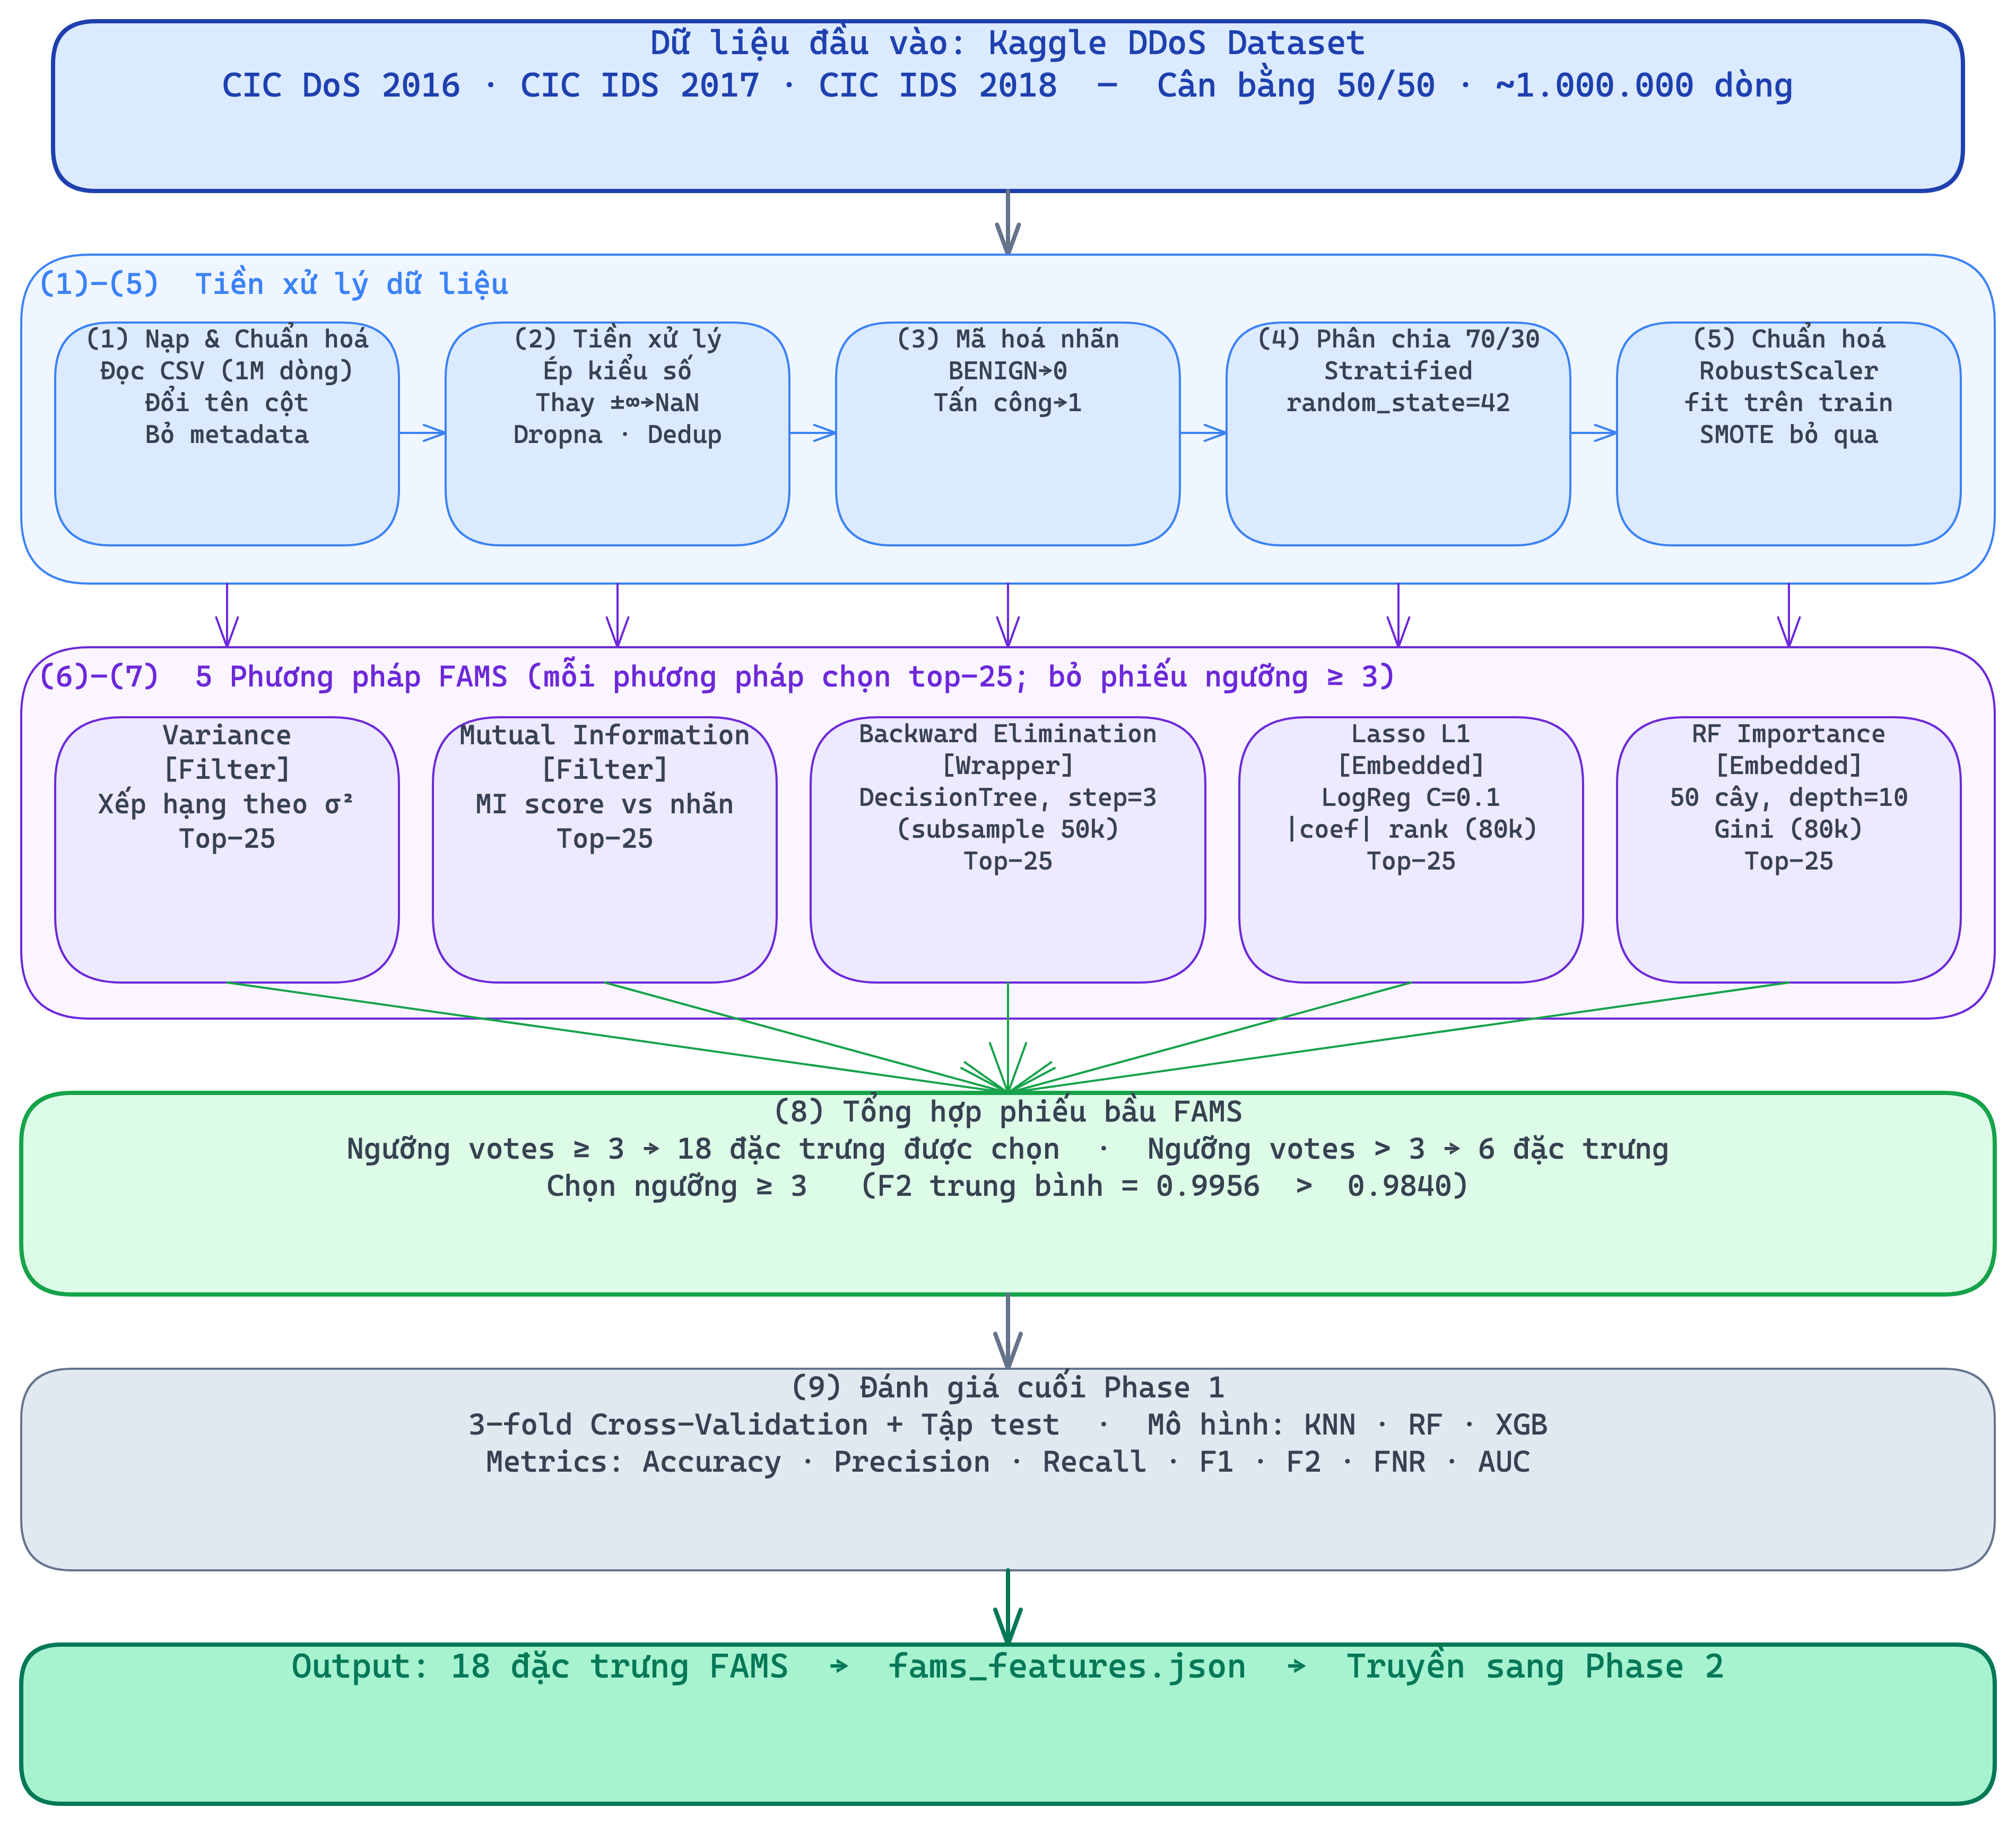
\includegraphics[width=\linewidth,keepaspectratio=true]{hinh/phase1_diagram_excalidraw.png}
\caption{Phase 1 -- Lựa chọn đặc trưng FAMS: từ dữ liệu Kaggle đến tập đặc trưng tối ưu.}
\label{fig:phase1_diagram}
\end{figure}

\begin{figure}[H]
\centering
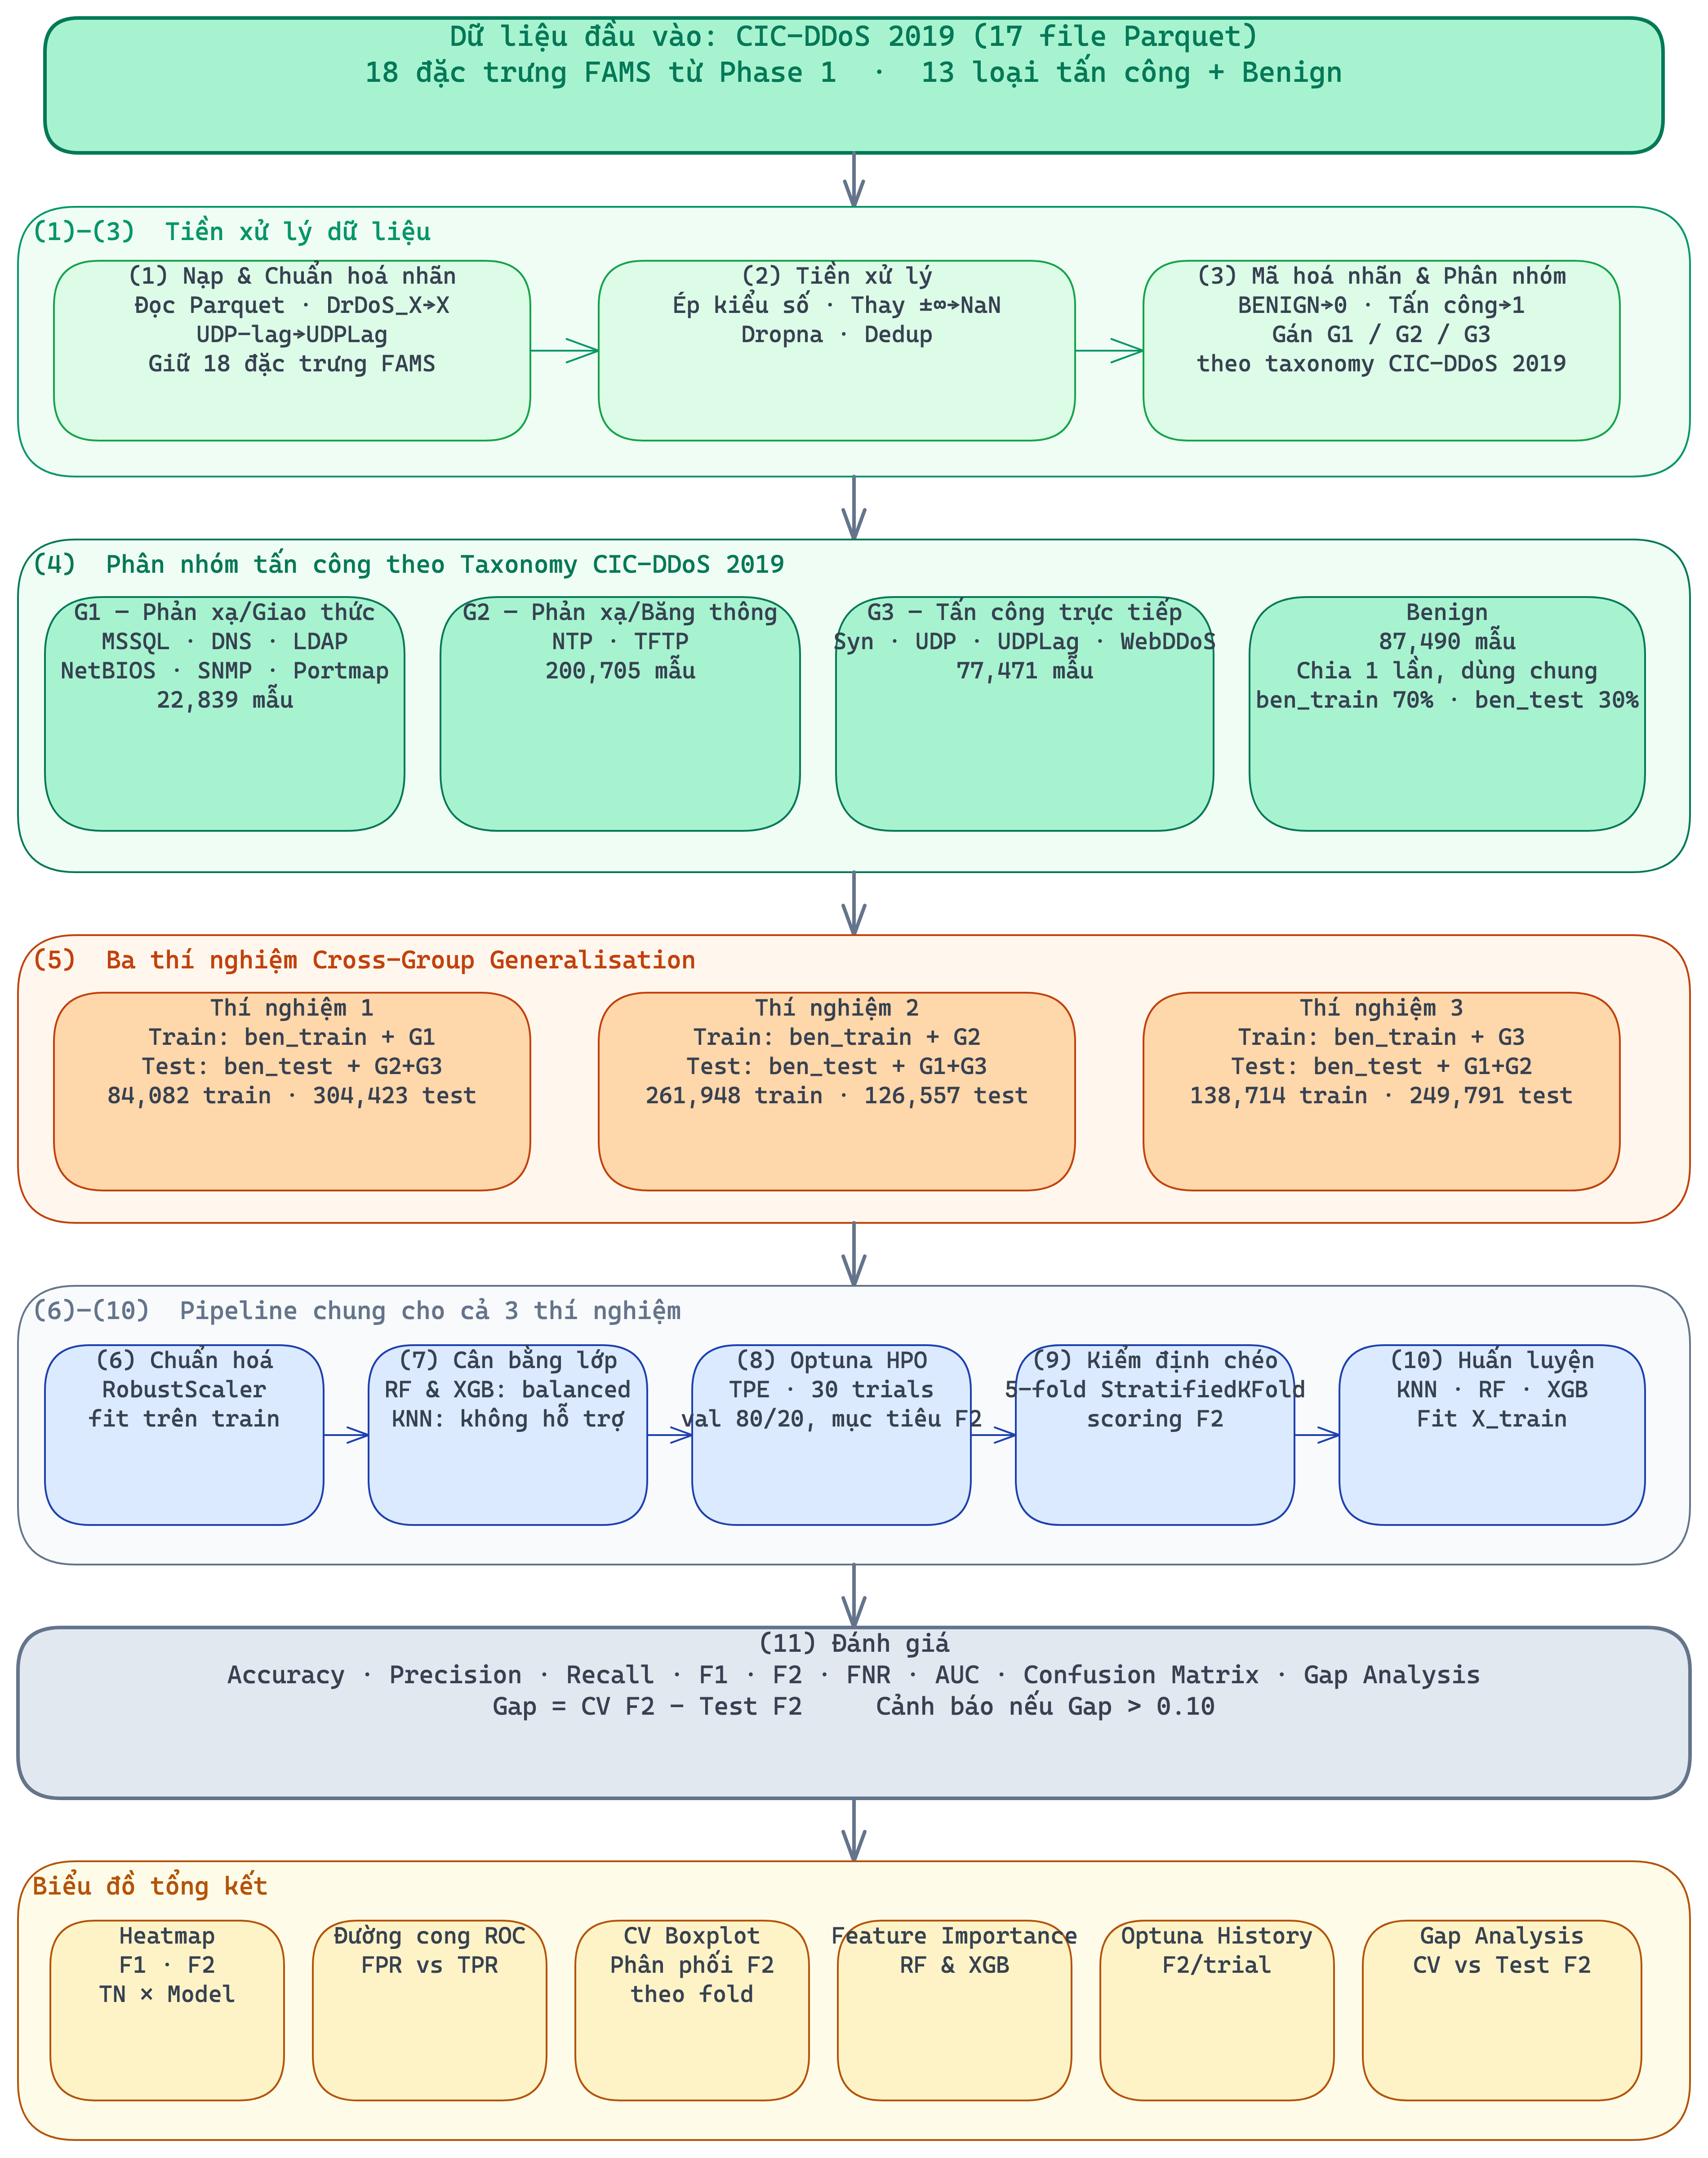
\includegraphics[width=\linewidth,keepaspectratio=true]{hinh/phase2_diagram_excalidraw.png}
\caption{Phase 2 -- Huấn luyện và đánh giá theo nhóm tấn công (Leave-One-Group-Out).}
\label{fig:phase2_diagram}
\end{figure}

\subsection{Dữ liệu và tiền xử lý}

\subsubsection{Bộ dữ liệu Phase 1 (Kaggle)}

Bộ dữ liệu tổng hợp từ Kaggle~\cite{kaggle_ddos_dataset} gộp lưu lượng từ ba bộ CIC DoS 2016, CIC IDS 2017 và CIC IDS 2018 thành một tập dữ liệu đã được cân bằng và chuẩn hóa nhãn. Đây là bộ dữ liệu flow-based với hơn 70 đặc trưng mô tả các thuộc tính thống kê của luồng mạng (kích thước gói tin, thời gian giữa các gói, số gói theo chiều forward/backward, v.v.). Sự đa dạng về loại lưu lượng của bộ này -- bao gồm nhiều kiểu DoS/DDoS cùng lưu lượng bình thường -- làm cho nó phù hợp cho bước lựa chọn đặc trưng.

\subsubsection{Bộ dữ liệu Phase 2 (CIC-DDoS 2019)}

CIC-DDoS 2019~\cite{cicddos2019} được tạo bởi Canadian Institute for Cybersecurity, cung cấp lưu lượng mạng flow-based ở định dạng Parquet gồm 17 file, tương ứng với nhiều loại tấn công DDoS hiện đại và lưu lượng bình thường (phân loại đầy đủ trong Hình~\ref{fig:cicddos2019_taxonomy}).

\begin{figure}[H]
\centering
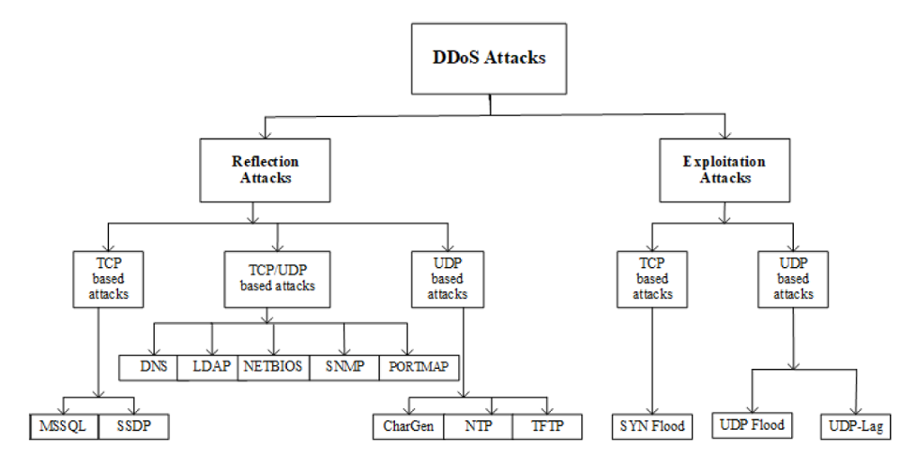
\includegraphics[width=\linewidth,keepaspectratio=true]{hinh/cicddos2019_taxonomy.png}
\caption{Phân loại tấn công DDoS trong bộ dữ liệu CIC-DDoS 2019~\cite{cicddos2019}.}
\label{fig:cicddos2019_taxonomy}
\end{figure} Sau tiền xử lý (loại bỏ hàng NaN, trùng lặp, và ép kiểu), bộ dữ liệu còn \textbf{388.505 dòng} (từ 431.371 dòng thô), bao gồm ba nhóm tấn công chính được sử dụng trong thiết kế thực nghiệm:
\begin{itemize}
    \item \textbf{G1 -- Reflection/Application:} MSSQL, DNS, LDAP, NetBIOS, SNMP, Portmap (22.839 mẫu tấn công).
    \item \textbf{G2 -- Reflection/Volume:} NTP, TFTP (200.705 mẫu).
    \item \textbf{G3 -- Exploitation:} Syn, UDP, UDPLag, WebDDoS (77.471 mẫu).
\end{itemize}
Lưu lượng Benign gồm \textbf{87.490 mẫu}, được chia ngẫu nhiên một lần theo tỷ lệ 70/30 (61.243 train / 26.247 test) và sử dụng chung cho cả ba thí nghiệm để đảm bảo tính nhất quán so sánh và tránh rò rỉ dữ liệu.

\subsubsection{Quy trình tiền xử lý chung}

Với cả hai bộ dữ liệu, quy trình tiền xử lý bao gồm:
\begin{enumerate}
    \item \textbf{Loại bỏ cột định danh:} Xóa các trường IP nguồn/đích, cổng, timestamp vì không mang thông tin tổng quát.
    \item \textbf{Xử lý giá trị thiếu và trùng lặp:} Loại bỏ hàng NaN và hàng trùng lặp hoàn toàn.
    \item \textbf{Chuẩn hóa nhãn:} Đưa nhãn về dạng thống nhất (ví dụ DrDoS\_DNS $\to$ DNS, UDP-lag $\to$ UDPLag).
    \item \textbf{Chuẩn hóa đặc trưng:} Áp dụng \textbf{RobustScaler}~\cite{pedregosa2011scikit} -- fit trên tập train, transform cả train và test -- để tránh data leakage và xử lý ngoại lai.
\end{enumerate}

\subsection{Thiết kế thực nghiệm: Leave-One-Group-Out}

Thiết kế thực nghiệm trung tâm của báo cáo là \textbf{Leave-One-Group-Out (LOGO)}: lần lượt sử dụng mỗi nhóm tấn công làm tập huấn luyện, trong khi các nhóm còn lại tạo thành tập kiểm thử. Cách tiếp cận này cho phép đánh giá trực tiếp \textit{khả năng tổng quát hóa liên nhóm} -- tức là mô hình học được từ một loại tấn công có phát hiện được các loại tấn công khác chưa từng thấy hay không.

Ba thí nghiệm được thiết kế như sau:
\begin{enumerate}
    \item \textbf{Exp 1:} Huấn luyện trên G1 + Benign (train) $\to$ Kiểm thử trên G2 + G3 + Benign (test).\\
    Kích thước: Train 84.082; Test 304.423.
    \item \textbf{Exp 2:} Huấn luyện trên G2 + Benign (train) $\to$ Kiểm thử trên G1 + G3 + Benign (test).\\
    Kích thước: Train 261.948; Test 126.557.
    \item \textbf{Exp 3:} Huấn luyện trên G3 + Benign (train) $\to$ Kiểm thử trên G1 + G2 + Benign (test).\\
    Kích thước: Train 138.714; Test 249.791.
\end{enumerate}

Trong mỗi thí nghiệm, tập Benign train được lấy từ phần 70\% đã chia cố định trước; tập Benign test là phần 30\% còn lại. Tập tấn công của nhóm huấn luyện được chia 70/30 theo stratified sampling~\cite{pedregosa2011scikit} để tạo tập train và tập validation nội bộ.

\subsection{Quy trình huấn luyện và tối ưu siêu tham số}

Với mỗi thí nghiệm và mỗi mô hình, quy trình huấn luyện gồm các bước:

\begin{enumerate}
    \item \textbf{Tối ưu siêu tham số bằng Optuna:} 30 trials với sampler TPE, mục tiêu tối đa hóa \textbf{F2-score} trung bình qua Stratified 5-Fold CV trên tập train. Tham số không gian tìm kiếm phụ thuộc mô hình (ví dụ: $k$ và metric khoảng cách cho KNN; số cây, độ sâu, số đặc trưng cho RF; learning rate, max depth, số rounds cho XGB).

    \item \textbf{Xử lý mất cân bằng lớp:} RF sử dụng \texttt{class\_weight='balanced'}; XGB dùng \texttt{scale\_pos\_weight} tỷ lệ nghịch với tần suất lớp; KNN không hỗ trợ cơ chế cân bằng lớp tường minh.

    \item \textbf{Huấn luyện mô hình cuối:} Sau khi tìm được siêu tham số tốt nhất, mô hình được huấn luyện lại trên \textit{toàn bộ} tập train (không chia fold).

    \item \textbf{Đánh giá trên tập test:} Mô hình được đánh giá trên tập test chứa các nhóm tấn công chưa thấy trong huấn luyện.
\end{enumerate}

\subsection{Chỉ số đánh giá}

Báo cáo sử dụng bộ chỉ số đánh giá sau, tính trên tập test hold-out:

\begin{itemize}
    \item \textbf{Accuracy:} Tỷ lệ dự đoán đúng tổng thể. Không phù hợp là chỉ số duy nhất do mất cân bằng lớp.
    \item \textbf{Precision:} $P = TP / (TP + FP)$. Trong số các mẫu được dự đoán là tấn công, bao nhiêu thực sự là tấn công.
    \item \textbf{Recall:} $R = TP / (TP + FN)$. Trong số các mẫu tấn công thực tế, bao nhiêu được phát hiện.
    \item \textbf{F1-Score:} Trung bình điều hòa của Precision và Recall ($\beta = 1$).
    \item \textbf{F2-Score:} Trung bình điều hòa có trọng số ($\beta = 2$), ưu tiên Recall. Đây là chỉ số chính của báo cáo.
    \item \textbf{FNR} (False Negative Rate): $FNR = FN / (FN + TP)$. Tỷ lệ tấn công bị bỏ sót; FNR càng thấp càng tốt.
    \item \textbf{AUC} (Area Under ROC Curve): Đánh giá khả năng phân biệt tổng thể của mô hình trên mọi ngưỡng quyết định.
    \item \textbf{Gap} $= \text{CV F2} - \text{Test F2}$: Chênh lệch giữa F2 nội bộ (cross-validation trên train) và F2 trên tập test. Gap dương lớn phản ánh mô hình overfit vào loại tấn công trong tập huấn luyện và tổng quát hóa kém.
    \item \textbf{Thời gian huấn luyện} (Training Time, giây): Thời gian huấn luyện mô hình cuối trên toàn bộ tập train sau khi đã tìm được siêu tham số tối ưu. Phản ánh chi phí tính toán offline của pipeline.
    \item \textbf{Thời gian suy luận} (Inference Time, ms/mẫu): Thời gian trung bình để mô hình phân loại một mẫu lưu lượng. Có ý nghĩa trực tiếp với yêu cầu phát hiện thời gian thực. Việc giảm số đặc trưng đầu vào từ 70+ xuống 18 (FAMS) kỳ vọng rút ngắn đáng kể chỉ số này, đặc biệt với KNN có chi phí suy luận tuyến tính theo số chiều.
\end{itemize}

\section{Thực nghiệm và đánh giá kết quả}
\label{sec:thuc-nghiem}

Chương này trình bày kết quả cụ thể của hai giai đoạn trong pipeline, bao gồm kết quả lựa chọn đặc trưng (Phase 1) và kết quả huấn luyện/đánh giá mô hình theo thiết kế Leave-One-Group-Out (Phase 2). Các kết quả số được trích xuất từ notebook \href{https://github.com/hoainn/HocMayATTT/blob/main/phase1\_feature\_selection.ipynb}{\texttt{phase1\_feature\_selection.ipynb}} và \href{https://github.com/hoainn/HocMayATTT/blob/main/phase2\_model\_training.ipynb}{\texttt{phase2\_model\_training.ipynb}}. Sơ đồ chi tiết pipeline đã được trình bày trong Hình~\ref{fig:phase1_diagram} và Hình~\ref{fig:phase2_diagram} (Chương~\ref{sec:phuong-phap}).

\subsection{Kết quả Phase 1: Lựa chọn đặc trưng FAMS}

\subsubsection{So sánh hai ngưỡng bỏ phiếu}

Phase 1 áp dụng khung FAMS với hai ngưỡng bỏ phiếu để xác định tập đặc trưng phù hợp nhất cho Phase 2. Mỗi phương pháp trong 5 phương pháp (Variance, Mutual Information, RFE, Lasso L1, RF Importance) chọn top-25 đặc trưng; hai ngưỡng được so sánh:

\begin{itemize}
    \item \textbf{Votes $\geq 3$:} Đặc trưng được chọn bởi ít nhất 3/5 phương pháp $\to$ \textbf{18 đặc trưng}.
    \item \textbf{Votes $> 3$:} Đặc trưng được chọn bởi ít nhất 4/5 phương pháp $\to$ \textbf{6 đặc trưng}.
\end{itemize}

Bảng~\ref{tab:phase1_eval} so sánh hiệu năng phân loại của ba mô hình trên tập test của bộ Kaggle với hai ngưỡng này.

\begin{table*}[!t]
\caption{So sánh hiệu năng theo ngưỡng bỏ phiếu FAMS trên bộ dữ liệu Kaggle.}
\label{tab:phase1_eval}
\begin{center}
\begin{adjustbox}{width=\textwidth}
\begin{tabular}{|l|l|r|r|r|r|r|r|r|}
\hline
\textbf{Ngưỡng} & \textbf{Mô hình} & \textbf{CV F1} & \textbf{Accuracy} & \textbf{Precision} & \textbf{Recall} & \textbf{F1} & \textbf{F2} & \textbf{FNR} \\
\hline
\multicolumn{9}{|l|}{\textit{Votes $\geq 3$ --- 18 đặc trưng}} \\
\hline
votes $\geq 3$ & KNN & 0,9927$\pm$0,0000 & 0,9930 & 0,9916 & 0,9939 & 0,9927 & 0,9934 & 0,0061 \\
               & RF  & 0,9971$\pm$0,0000 & 0,9972 & 0,9976 & 0,9966 & 0,9971 & 0,9968 & 0,0034 \\
               & XGB & 0,9971$\pm$0,0001 & 0,9972 & 0,9980 & 0,9961 & 0,9971 & 0,9965 & 0,0039 \\
\hline
\multicolumn{9}{|l|}{\textit{Votes $> 3$ --- 6 đặc trưng}} \\
\hline
votes $> 3$    & KNN & 0,9824$\pm$0,0002 & 0,9828 & 0,9777 & 0,9866 & 0,9821 & 0,9848 & 0,0134 \\
               & RF  & 0,9809$\pm$0,0003 & 0,9818 & 0,9808 & 0,9812 & 0,9810 & 0,9811 & 0,0188 \\
               & XGB & 0,9827$\pm$0,0003 & 0,9832 & 0,9769 & 0,9883 & 0,9826 & 0,9860 & 0,0117 \\
\hline
\end{tabular}
\end{adjustbox}
\end{center}
\end{table*}

F2 trung bình (trung bình ba mô hình) với ngưỡng $\geq 3$ đạt \textbf{0,9956}, cao hơn \textbf{0,9840} với ngưỡng $> 3$. Sự chênh lệch này cho thấy 12 đặc trưng bổ sung khi hạ ngưỡng từ $>3$ xuống $\geq 3$ mang lại thông tin có giá trị, đặc biệt thể hiện qua chỉ số FNR giảm đáng kể (ví dụ RF từ 0,0188 xuống 0,0034). Do đó, \textbf{tập 18 đặc trưng (votes $\geq 3$)} được chọn để sử dụng trong Phase 2.

Bảng~\ref{tab:fams_features} liệt kê 18 đặc trưng được chọn sau bước bỏ phiếu FAMS.

\begin{table}[H]
\caption{18 đặc trưng được chọn bởi FAMS (votes $\geq 3$).}
\label{tab:fams_features}
\begin{center}
\begin{tabular}{|c|l|}
\hline
\textbf{STT} & \textbf{Tên đặc trưng} \\
\hline
1  & Fwd Packet Length Mean \\
2  & Fwd Packet Length Max \\
3  & Fwd Packets Length Total \\
4  & Fwd Seg Size Min \\
5  & Flow IAT Min \\
6  & Fwd Packet Length Std \\
7  & Subflow Bwd Bytes \\
8  & Packet Length Max \\
9  & Init Bwd Win Bytes \\
10 & Packet Length Std \\
11 & Subflow Fwd Bytes \\
12 & Fwd Header Length \\
13 & Flow Packets/s \\
14 & Bwd Packet Length Max \\
15 & Bwd Packets Length Total \\
16 & Avg Fwd Segment Size \\
17 & Subflow Fwd Packets \\
18 & Bwd Packet Length Std \\
\hline
\end{tabular}
\end{center}
\end{table}

\subsection{Kết quả Phase 2: Leave-One-Group-Out trên CIC-DDoS 2019}

\subsubsection{Kết quả tổng hợp}

Bảng~\ref{tab:phase2_results} trình bày đầy đủ kết quả của ba thí nghiệm LOGO trên bộ CIC-DDoS 2019 với 18 đặc trưng FAMS. Với mỗi thí nghiệm, CV F2 phản ánh hiệu năng nội bộ (trên tập train qua 5-fold CV), trong khi Test F2 phản ánh khả năng tổng quát hóa sang các nhóm tấn công chưa thấy. Chỉ số \textbf{Gap} = CV F2 $-$ Test F2 định lượng mức độ overfit theo nhóm tấn công.

\begin{table*}[!t]
\caption{Kết quả Leave-One-Group-Out trên CIC-DDoS 2019.}
\label{tab:phase2_results}
\begin{center}
\begin{adjustbox}{width=\textwidth}
\begin{tabular}{|l|l|r|r|r|r|r|r|r|}
\hline
\textbf{Thí nghiệm} & \textbf{Mô hình} & \textbf{CV F2} & \textbf{Test F2} & \textbf{Test F1} & \textbf{Recall} & \textbf{FNR} & \textbf{AUC} & \textbf{Gap} \\
\hline
Exp 1 (G1$\to$G2+G3) & KNN & 0,9952$\pm$0,0009 & 0,6027 & 0,7081 & 0,5482 & 0,4518 & 0,7733 & +0,3925 \\
                      & RF  & 0,9972$\pm$0,0006 & 0,8332 & 0,8888 & 0,7999 & 0,2001 & 0,9844 & +0,1640 \\
                      & XGB & 0,9976$\pm$0,0005 & 0,7764 & 0,8474 & 0,7353 & 0,2647 & 0,9887 & +0,2212 \\
\hline
Exp 2 (G2$\to$G1+G3) & KNN & 0,9989$\pm$0,0002 & 0,6109 & 0,7150 & 0,5568 & 0,4432 & 0,8013 & +0,3880 \\
                      & RF  & 0,9995$\pm$0,0001 & 0,6196 & 0,7226 & 0,5658 & 0,4342 & 0,8047 & +0,3799 \\
                      & XGB & 0,9993$\pm$0,0002 & 0,6221 & 0,7247 & 0,5684 & 0,4316 & 0,8989 & +0,3772 \\
\hline
Exp 3 (G3$\to$G1+G2) & KNN & 0,9937$\pm$0,0007 & 0,9171 & 0,9462 & 0,8987 & 0,1013 & 0,9453 & +0,0766 \\
                      & RF  & 0,9981$\pm$0,0004 & \textbf{0,9848} & \textbf{0,9904} & \textbf{0,9811} & \textbf{0,0189} & 0,9990 & +0,0133 \\
                      & XGB & 0,9978$\pm$0,0002 & 0,9022 & 0,9364 & 0,8807 & 0,1193 & 0,9981 & +0,0956 \\
\hline
\end{tabular}
\end{adjustbox}
\end{center}
\end{table*}

\subsubsection{Phân tích Exp 1 -- Huấn luyện trên G1 (Reflection/Application)}

Khi huấn luyện trên nhóm G1 (MSSQL, DNS, LDAP, NetBIOS, SNMP, Portmap -- chỉ 22.839 mẫu tấn công), Test F2 giảm đáng kể so với CV F2: KNN đạt 0,60 (Gap +0,39), RF đạt 0,83 (Gap +0,16), XGB đạt 0,78 (Gap +0,22). Điều này cho thấy mô hình học được đặc trưng gắn với lưu lượng phản xạ giao thức ứng dụng, nhưng không tổng quát hóa tốt sang tấn công thể tích (G2: NTP/TFTP) hay tấn công khai thác (G3: Syn/UDP/WebDDoS).

Nhóm G1 có kích thước nhỏ nhất trong ba nhóm tấn công -- chỉ 22.839 mẫu, bằng khoảng 26\% so với lưu lượng Benign -- và có đặc trưng đồng nhất về giao thức (DNS, LDAP, MSSQL đều là phản xạ ứng dụng), dẫn đến việc mô hình học ``nhận dạng giao thức cụ thể'' hơn là pattern DDoS tổng quát. RF tổng quát hóa tốt hơn KNN và XGB trong thí nghiệm này, với FNR 0,20 so với 0,45 (KNN) và 0,26 (XGB), cho thấy cơ chế bagging giúp giảm thiểu một phần sự phụ thuộc vào đặc trưng giao thức khi dữ liệu đủ đa dạng trong mỗi cây.

\subsubsection{Phân tích Exp 2 -- Huấn luyện trên G2 (Reflection/Volume)}

Exp 2 cho thấy một trường hợp đáng chú ý: mặc dù G2 có kích thước lớn nhất (200.705 mẫu tấn công, chủ yếu NTP và TFTP), cả ba mô hình đều có Gap lớn tương đương nhau (0,38--0,39) và Test F2 thấp (0,61--0,62). CV F2 cực kỳ cao (RF: 0,9995) cho thấy mô hình phân loại hoàn hảo lưu lượng NTP/TFTP vs Benign trong nội bộ, nhưng không tổng quát hóa được sang các loại tấn công khác.

Điểm đáng chú ý là trong Exp 2, lợi thế bagging của RF biến mất hoàn toàn -- RF, XGB và KNN hội tụ về cùng một mức Gap (0,38--0,39). Điều này có thể giải thích như sau: NTP và TFTP có đặc trưng rất đặc thù (kích thước phản hồi lớn bất thường, cổng UDP 123/69), khiến \textit{toàn bộ} 200.705 mẫu huấn luyện phân bố trong một vùng đặc trưng hẹp, đồng nhất. Khi tập bootstrap của mỗi cây trong RF đều rút từ cùng vùng đặc thù này, mọi cây đều học cùng một biên quyết định hẹp theo giao thức -- cơ chế bagging không còn tạo ra sự đa dạng giữa các cây vì dữ liệu nguồn thiếu đa dạng. Kết quả này nhấn mạnh rằng \textit{kích thước tập huấn luyện lớn không đảm bảo tổng quát hóa tốt nếu tập đó thiếu đa dạng về loại lưu lượng}.

\subsubsection{Phân tích Exp 3 -- Huấn luyện trên G3 (Exploitation)}

Exp 3 cho kết quả vượt trội so với hai thí nghiệm còn lại. RF đạt Test F2 = \textbf{0,9848} với Gap = +0,013 -- gần như không có hiện tượng overfit. KNN và XGB cũng cải thiện đáng kể (Test F2 lần lượt 0,92 và 0,90). Tỷ lệ bỏ sót tấn công (FNR) của RF chỉ \textbf{1,89\%}, tức là mô hình phát hiện được hơn 98\% các cuộc tấn công từ G1 và G2 mặc dù không được huấn luyện trên chúng.

Lý giải cho kết quả xuất sắc của Exp 3: Nhóm G3 bao gồm cả tấn công thể tích (UDP Flood, Syn Flood) và tầng ứng dụng (WebDDoS, UDPLag), tạo ra đặc trưng học đa dạng về kích thước gói tin, tốc độ luồng, và tỷ lệ gói tin forward/backward. Bộ dữ liệu Kaggle sử dụng trong Phase 1 cũng chứa UDP Flood và Syn Flood, nên tập đặc trưng FAMS được tối ưu hóa một phần cho các loại tấn công này, tạo ra sự tương thích tốt giữa đặc trưng học được và bài toán phân loại G3.

\subsection{Kết quả trực quan}

Hình~\ref{fig:phase2_heatmap} tóm tắt Test F2 của ba mô hình qua ba thí nghiệm.

\begin{figure}[H]
    \centering
    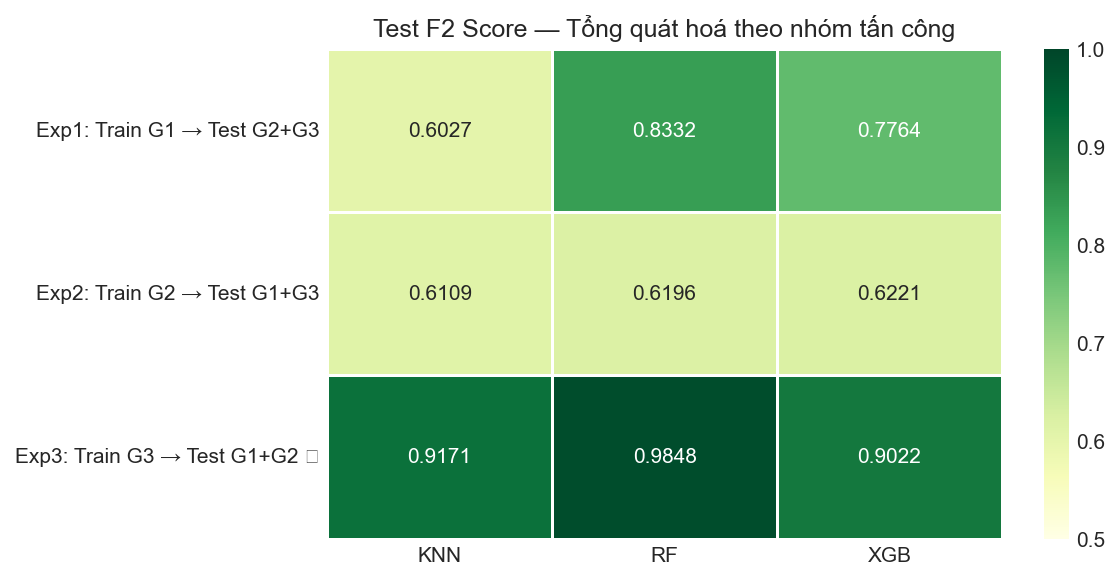
\includegraphics[width=\linewidth]{hinh/phase2_heatmap.png}
    \caption{Heatmap Test F2 theo thí nghiệm và mô hình.}
    \label{fig:phase2_heatmap}
\end{figure}

Heatmap cho thấy bất đối xứng rõ rệt giữa ba thí nghiệm: Exp 3 nổi bật ở góc phải trên, trong khi Exp 1 và Exp 2 đồng loạt thấp, gợi ý vấn đề tổng quát hóa xuất phát từ đặc tính của nhóm huấn luyện chứ không phải từ mô hình cụ thể.

Hình~\ref{fig:phase2_roc} thể hiện đường cong ROC trên tập test cho từng thí nghiệm.

\begin{figure}[H]
    \centering
    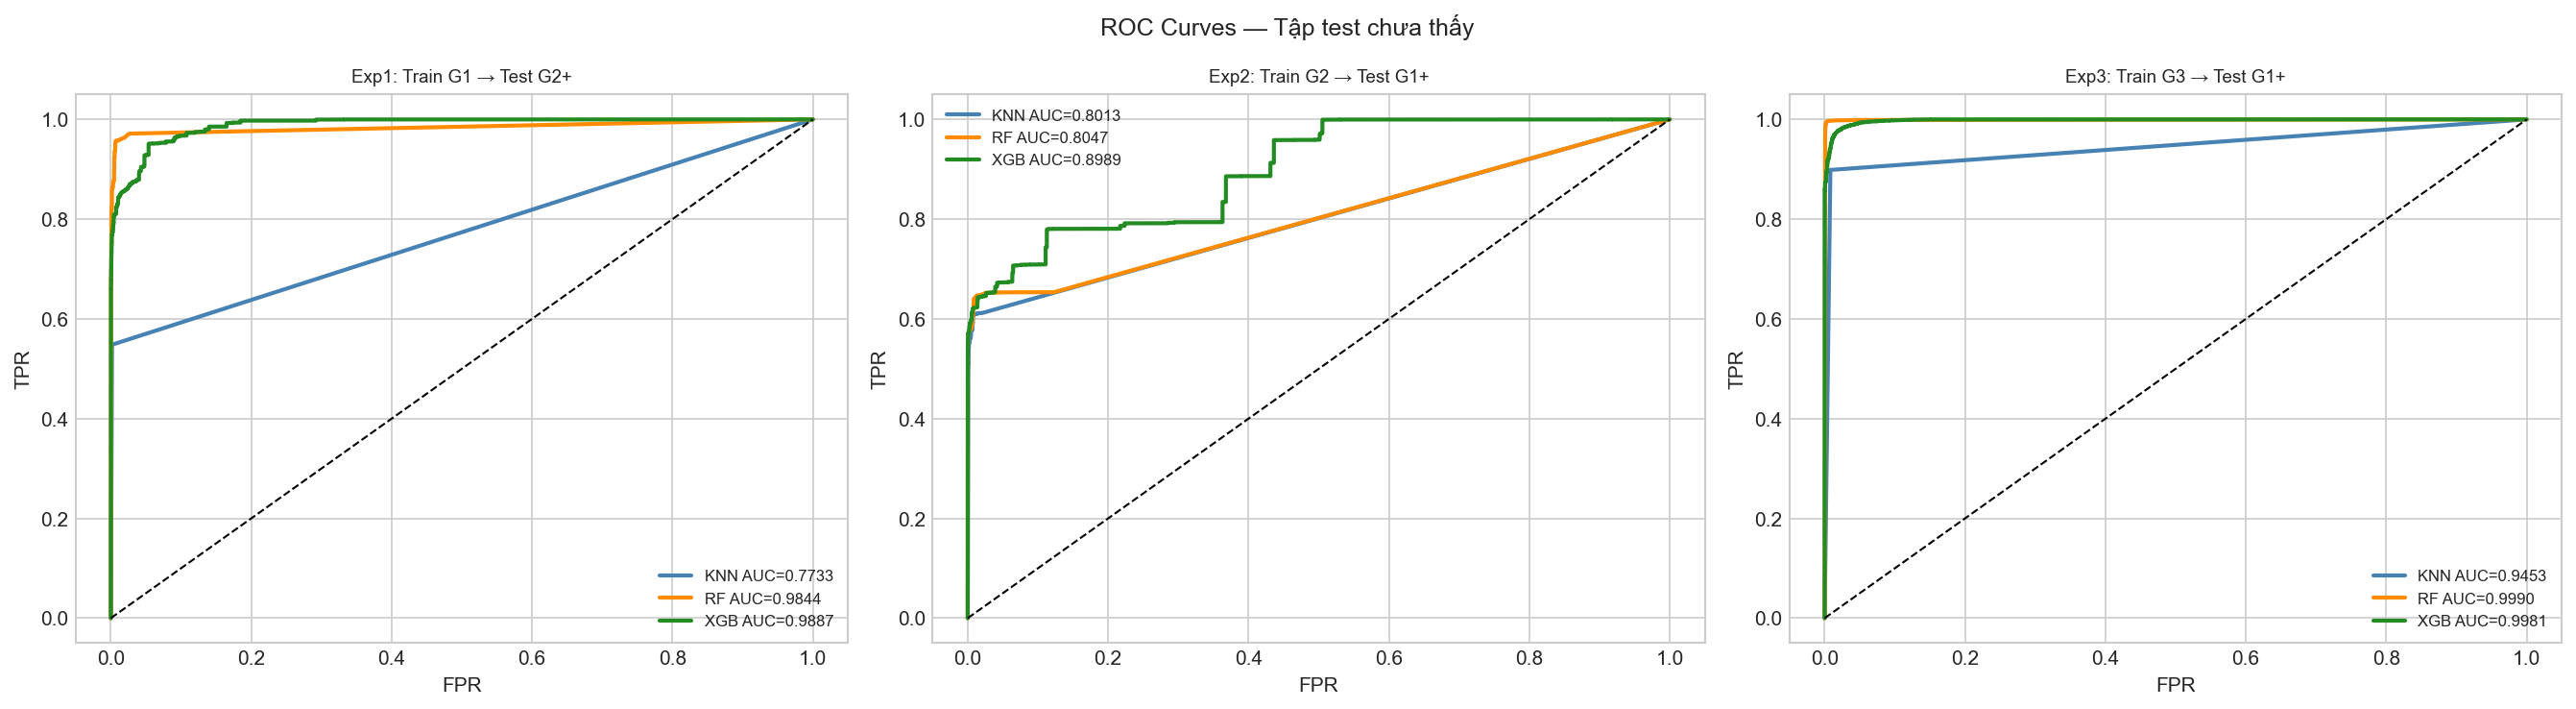
\includegraphics[width=\linewidth]{hinh/phase2_roc.png}
    \caption{Đường cong ROC trên tập test.}
    \label{fig:phase2_roc}
\end{figure}

Đường cong ROC tách biệt rõ Exp 3 (góc trên trái) so với Exp 1/2, xác nhận rằng sự suy giảm Test F2 phản ánh giới hạn hệ thống chứ không phải do ngưỡng phân loại. KNN ở Exp 1 và Exp 2 có AUC thấp nhất ($\approx$ 0,77--0,80), cho thấy bản thân xác suất phân loại cũng kém tin cậy ở những kịch bản này.

Hình~\ref{fig:phase2_confusion} thể hiện ma trận nhầm lẫn của mô hình tốt nhất mỗi thí nghiệm.

\begin{figure}[H]
    \centering
    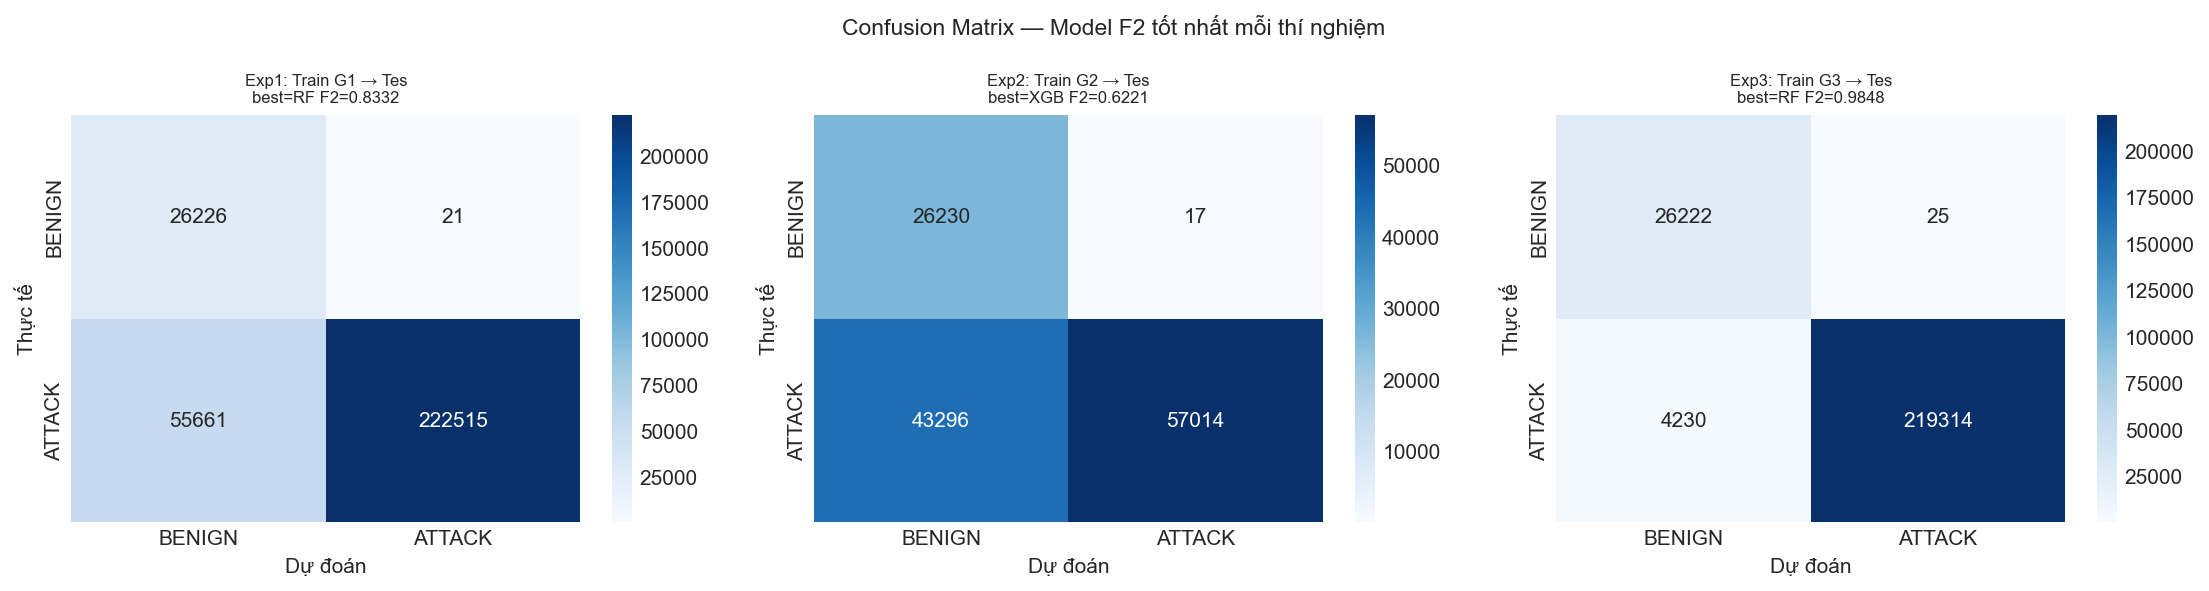
\includegraphics[width=\linewidth]{hinh/phase2_confusion_matrix.png}
    \caption{Ma trận nhầm lẫn của mô hình tốt nhất mỗi thí nghiệm.}
    \label{fig:phase2_confusion}
\end{figure}

Ma trận nhầm lẫn làm nổi bật nguồn gốc lỗi: ở Exp 1\&2, phần lớn lỗi là False Negative (tấn công bị phân loại là Benign), trái với Exp 3 nơi cả hai loại lỗi đều gần bằng không. Điều này xác nhận rằng mô hình không học được biên phân tách tổng quát khi tập huấn luyện đơn điệu về giao thức.

Hình~\ref{fig:phase2_cv_boxplot} thể hiện phân phối CV F2 qua 5 fold cho từng thí nghiệm.

\begin{figure}[H]
    \centering
    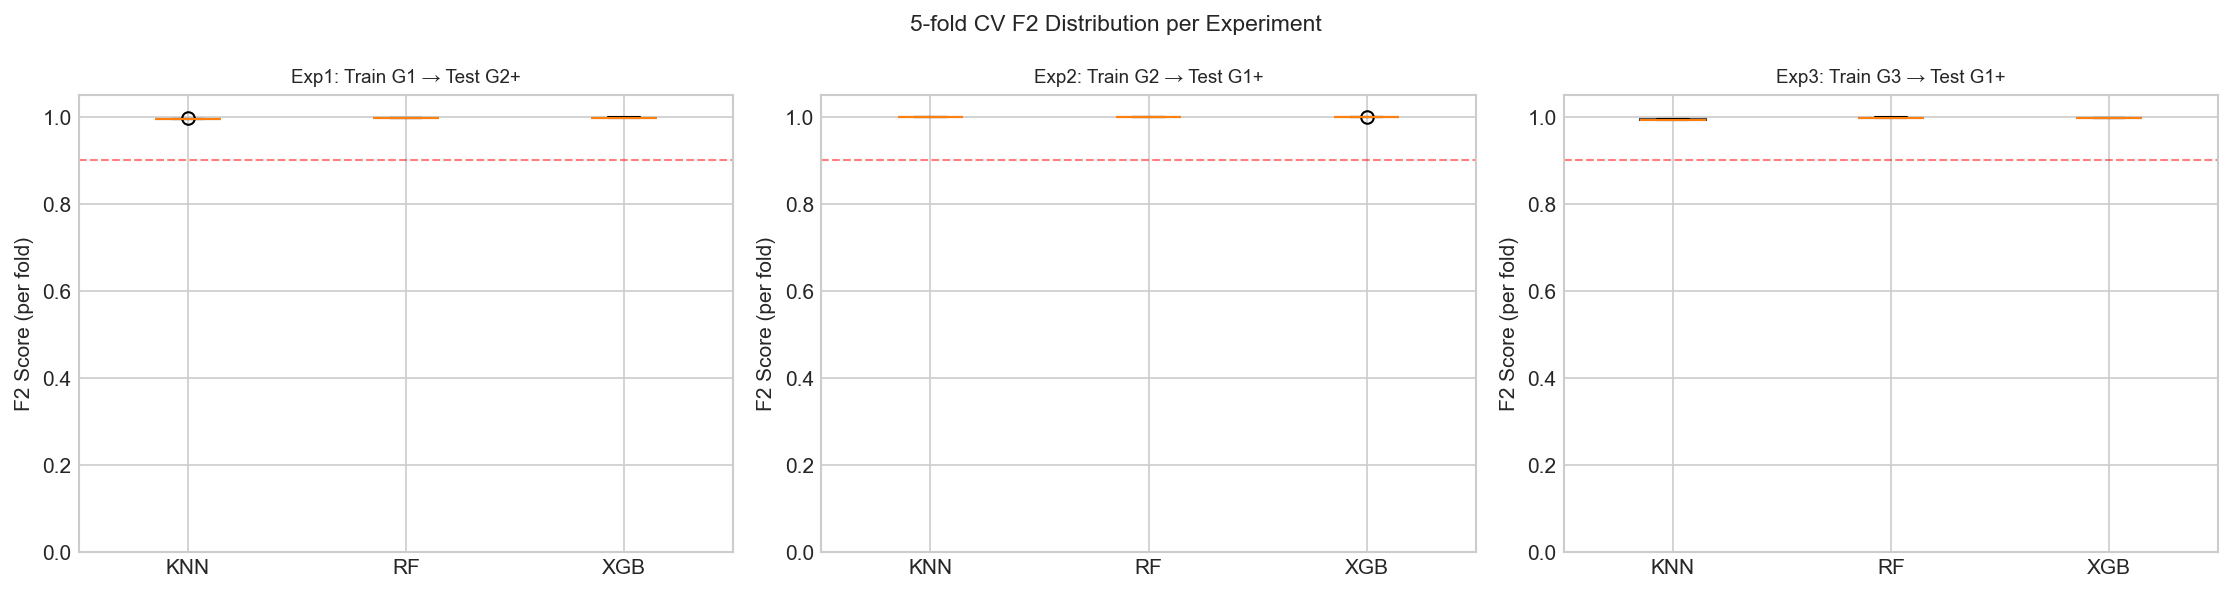
\includegraphics[width=\linewidth]{hinh/phase2_cv_boxplot.png}
    \caption{Phân phối CV F2 qua 5 fold theo từng thí nghiệm.}
    \label{fig:phase2_cv_boxplot}
\end{figure}

CV F2 rất ổn định (độ lệch chuẩn nhỏ) ở cả ba thí nghiệm, xác nhận rằng Gap lớn ở Exp 1\&2 xuất phát từ overfitting nhóm tấn công, không phải từ sự bất ổn của quá trình cross-validation.

Hình~\ref{fig:phase2_feature_importance} thể hiện feature importance của RF và XGB.

\begin{figure}[H]
    \centering
    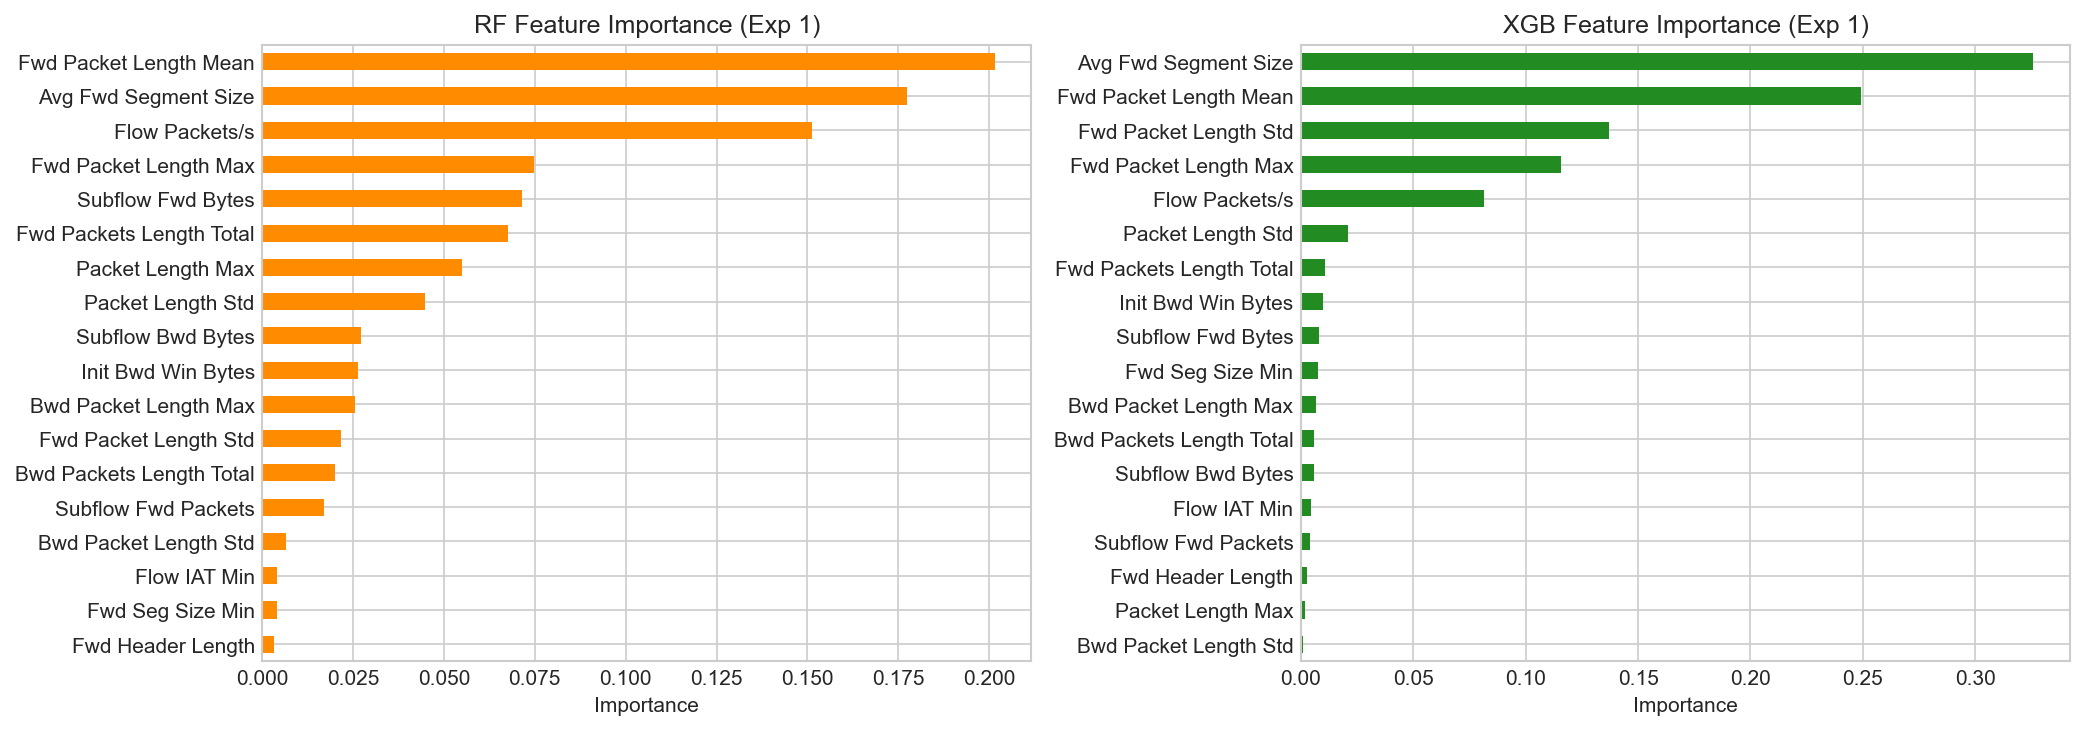
\includegraphics[width=\linewidth]{hinh/phase2_feature_importance.png}
    \caption{Feature importance của RF và XGB.}
    \label{fig:phase2_feature_importance}
\end{figure}

Các đặc trưng thể tích như \texttt{Fwd Packet Length Mean/Max}, \texttt{Flow IAT Max}, \texttt{Flow Bytes/s} chiếm tỷ trọng lớn trong cả RF và XGB, phù hợp với lý giải về sự tương đồng giữa G3 và bộ dữ liệu Kaggle.

Hình~\ref{fig:phase2_optuna_history} thể hiện lịch sử tối ưu Optuna theo số trial.

\begin{figure}[H]
    \centering
    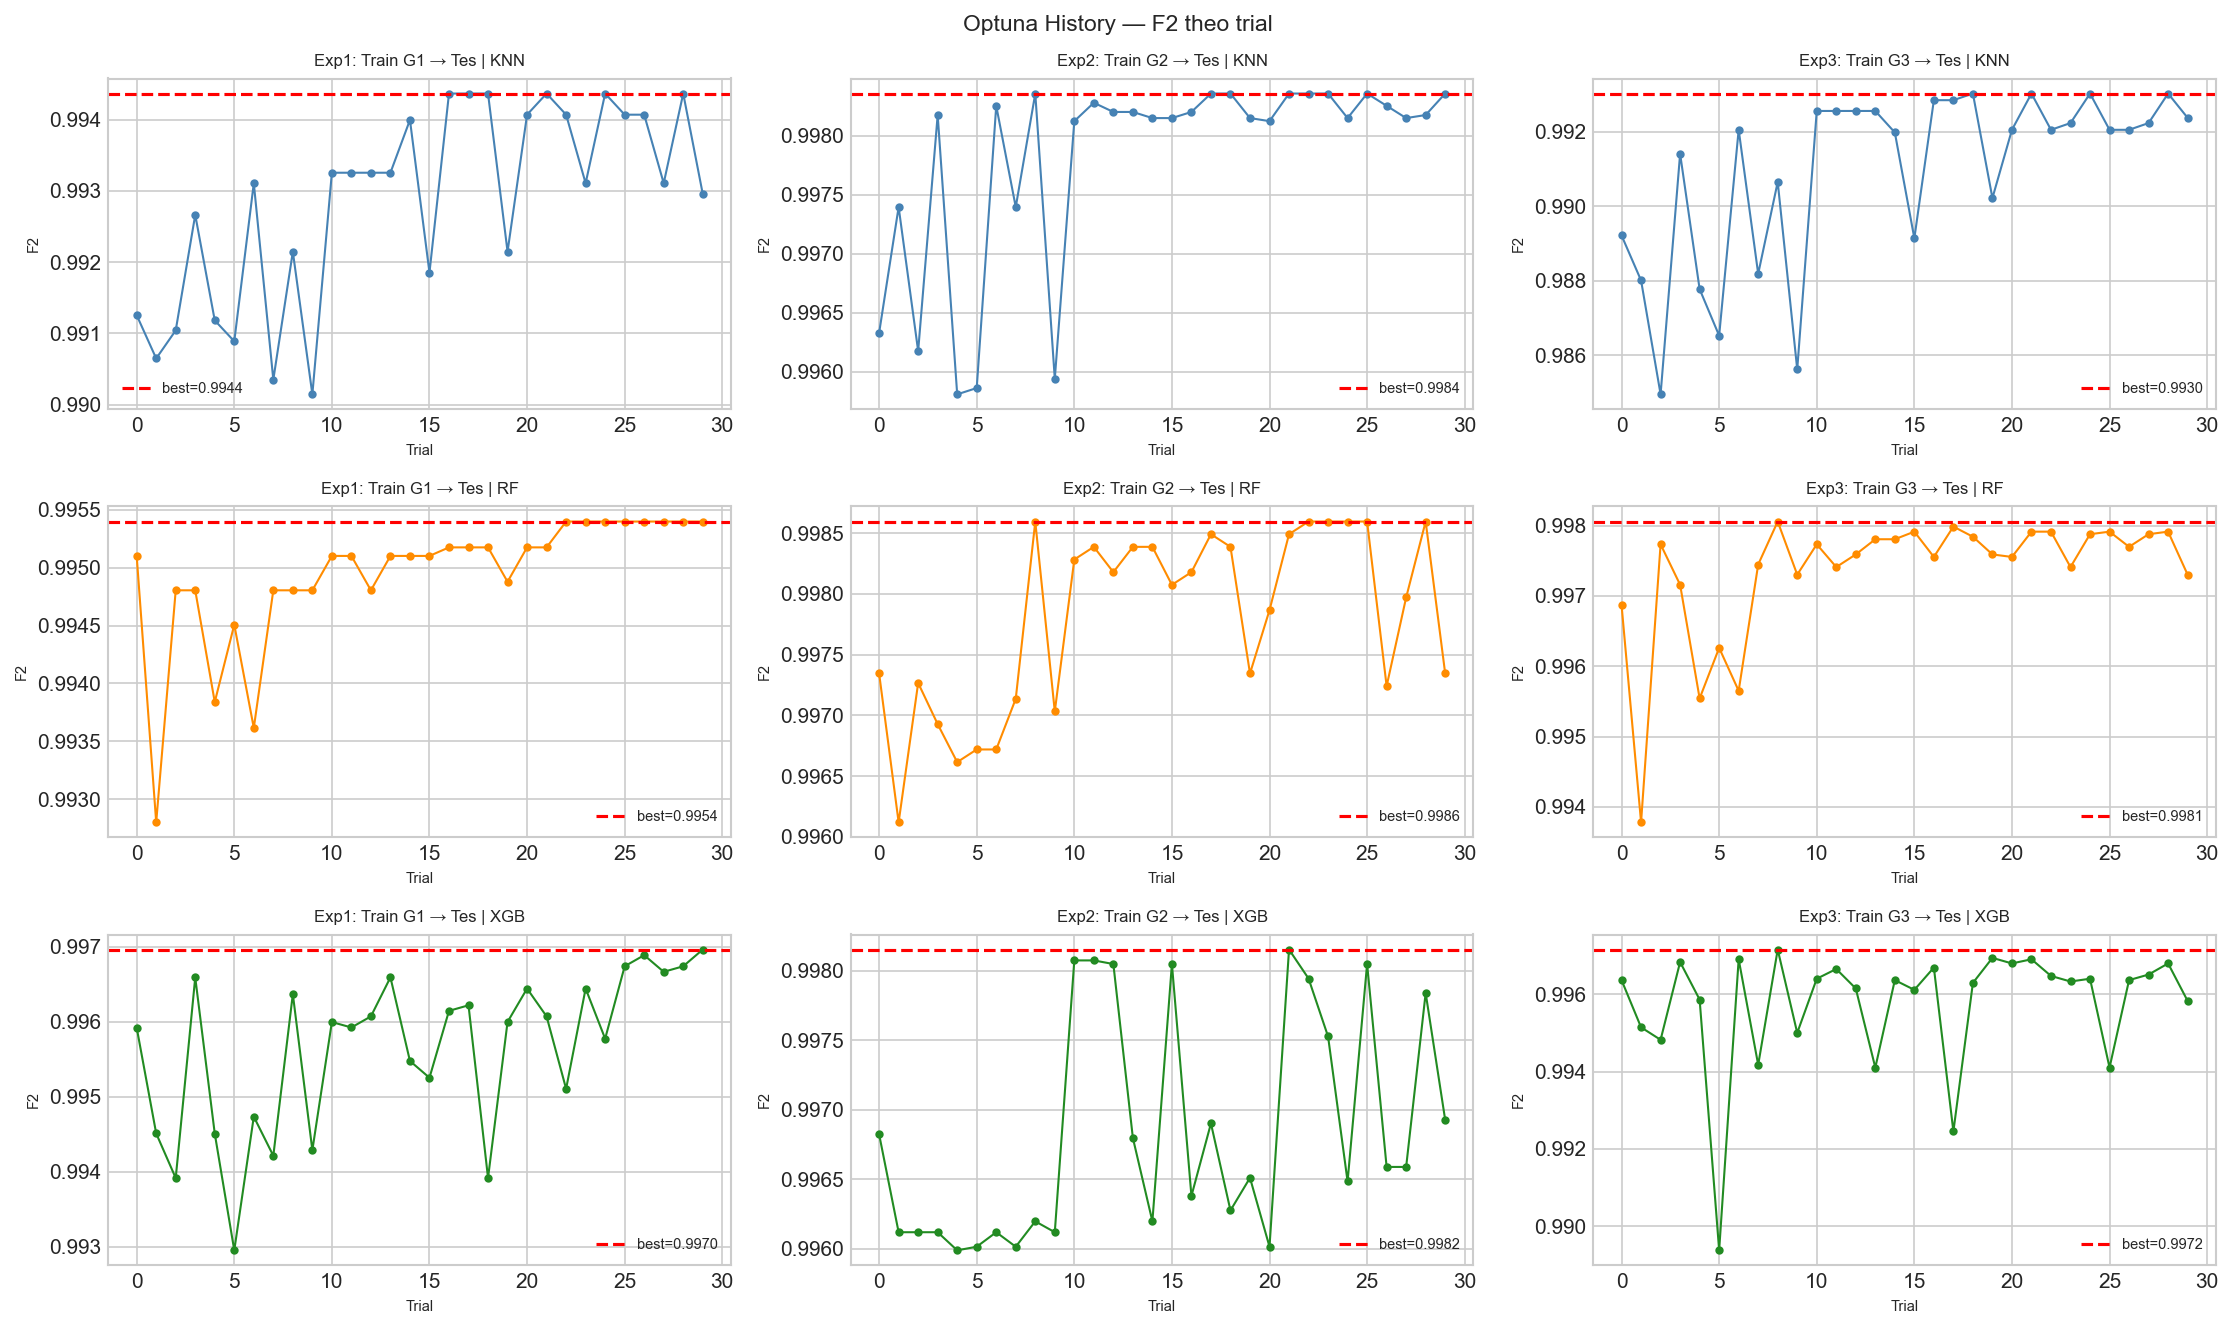
\includegraphics[width=\linewidth]{hinh/phase2_optuna_history.png}
    \caption{Lịch sử tối ưu Optuna theo số trial.}
    \label{fig:phase2_optuna_history}
\end{figure}

Optuna TPE hội tụ nhanh, thường tìm được siêu tham số tốt sau 10--15 trong tổng số 30 trial ở cả ba thí nghiệm.

Bảng~\ref{tab:optuna_params} liệt kê bộ siêu tham số tốt nhất mà Optuna tìm được cho từng mô hình và từng thí nghiệm.

\begin{table*}[!t]
\caption{Siêu tham số tốt nhất do Optuna TPE tìm được (30 trial, subsample 50.000 mẫu/trial). KNN cố định \texttt{algorithm=ball\_tree}; các tham số còn lại do Optuna tối ưu.}
\label{tab:optuna_params}
\begin{center}
\begin{adjustbox}{width=\textwidth}
\begin{tabular}{|l|l|l|}
\hline
\textbf{Thí nghiệm} & \textbf{Mô hình} & \textbf{Siêu tham số tốt nhất} \\
\hline
\multirow{3}{*}{Exp 1 (G1)} & KNN & \texttt{n\_neighbors=3, weights=distance} \\
 & RF  & \texttt{n\_estimators=100, max\_depth=19, min\_samples\_split=2, max\_features=log2} \\
 & XGB & \texttt{n\_estimators=500, max\_depth=7, learning\_rate=0.035, subsample=0.785, colsample\_bytree=0.744} \\
\hline
\multirow{3}{*}{Exp 2 (G2)} & KNN & \texttt{n\_neighbors=5, weights=distance} \\
 & RF  & \texttt{n\_estimators=150, max\_depth=18, min\_samples\_split=2, max\_features=log2} \\
 & XGB & \texttt{n\_estimators=450, max\_depth=7, learning\_rate=0.094, subsample=0.999, colsample\_bytree=0.816} \\
\hline
\multirow{3}{*}{Exp 3 (G3)} & KNN & \texttt{n\_neighbors=3, weights=distance} \\
 & RF  & \texttt{n\_estimators=500, max\_depth=15, min\_samples\_split=5, max\_features=log2} \\
 & XGB & \texttt{n\_estimators=200, max\_depth=6, learning\_rate=0.133, subsample=0.918, colsample\_bytree=0.820} \\
\hline
\end{tabular}
\end{adjustbox}
\end{center}
\end{table*}

\subsection{Đánh giá hiệu quả tính toán}

Một trong những mục tiêu quan trọng của bước lựa chọn đặc trưng FAMS là giảm số chiều đầu vào của mô hình, từ đó rút ngắn thời gian huấn luyện và suy luận. Bảng~\ref{tab:timing} trình bày thời gian huấn luyện và thời gian suy luận của ba mô hình trên ba thí nghiệm.

Về mặt lý thuyết, việc giảm từ 70+ đặc trưng xuống còn 18 đặc trưng (giảm $\approx$75\% số chiều) có tác động khác nhau tùy mô hình:
\begin{itemize}
    \item \textbf{KNN:} Hưởng lợi nhiều nhất vì chi phí suy luận tỷ lệ trực tiếp với số chiều $d$ -- tính khoảng cách Euclid trên 18 chiều nhanh hơn đáng kể so với 70+ chiều.
    \item \textbf{Random Forest \& XGBoost:} Giảm số chiều giúp rút ngắn thời gian tìm điểm chia tại mỗi nút cây, qua đó giảm thời gian huấn luyện; tác động đến suy luận ít hơn KNN nhưng vẫn có ý nghĩa khi tập test lớn.
\end{itemize}

\begin{table}[H]
\caption{Thời gian huấn luyện (s) và suy luận (ms/mẫu) của các mô hình theo từng thí nghiệm. KNN sử dụng \texttt{algorithm=ball\_tree} cố định để đảm bảo so sánh nhất quán.}
\label{tab:timing}
\begin{center}
\begin{adjustbox}{width=\linewidth}
\begin{tabular}{|l|l|r|r|r|r|}
\hline
\textbf{Thí nghiệm} & \textbf{Mô hình} & \textbf{Train size} & \textbf{T. huấn luyện (s)} & \textbf{T. suy luận (ms/mẫu)} & \textbf{Test F2} \\
\hline
Exp 1 (G1$\to$G2+G3) & KNN & 124.225 & 0,06 & 0,1102 & 0,5790 \\
                      & RF  & 124.225 & 1,00 & 0,0031 & 0,8330 \\
                      & XGB & 124.225 & 1,96 & 0,0013 & 0,7753 \\
\hline
Exp 2 (G2$\to$G1+G3) & KNN & 318.116 & 0,20 & 0,1526 & 0,5741 \\
                      & RF  & 318.116 & 2,53 & 0,0054 & 0,6032 \\
                      & XGB & 318.116 & 2,62 & 0,0009 & 0,6058 \\
\hline
Exp 3 (G3$\to$G1+G2) & KNN & 184.692 & 0,09 & 0,0559 & 0,9204 \\
                      & RF  & 184.692 & 5,73 & 0,0111 & 0,9870 \\
                      & XGB & 184.692 & 0,83 & 0,0005 & 0,9519 \\
\hline
\end{tabular}
\end{adjustbox}
\end{center}
\end{table}

\subsection{Tổng hợp và nhận xét}

\subsubsection{So sánh ba mô hình}

\textbf{Random Forest} là mô hình nhất quán nhất về khả năng tổng quát hóa: đạt Test F2 cao nhất ở Exp 1 (0,83) và Exp 3 (0,98), đồng thời có Gap nhỏ nhất ở Exp 3 (+0,013). Cơ chế bagging của RF giúp giảm phương sai và tránh overfit vào đặc trưng đặc thù của nhóm tấn công huấn luyện.

\textbf{XGBoost} đạt AUC cao (0,99 ở Exp 1 và Exp 3) nhưng có Gap lớn hơn RF ở Exp 3 (+0,096 so với +0,013). Điều này gợi ý XGBoost có xu hướng học các pattern phức tạp hơn của tập train, nhưng phần pattern đó không hoàn toàn chuyển giao sang nhóm tấn công mới.

\textbf{KNN} có Test F2 thấp nhất ở Exp 1 và Exp 2 (khoảng 0,61), nhưng cải thiện lên 0,92 ở Exp 3. Điều này phù hợp với đặc tính của KNN: hoạt động tốt khi phân phối dữ liệu train và test có sự tương đồng cao trong không gian đặc trưng (trường hợp Exp 3), nhưng kém khi phân phối khác biệt lớn.

\subsubsection{Ảnh hưởng của đặc trưng FAMS đến tổng quát hóa}

Kết quả thực nghiệm cho thấy tập 18 đặc trưng FAMS được tối ưu hóa cho bộ dữ liệu Kaggle (chứa nhiều tấn công thể tích như UDP Flood, Syn) phù hợp tốt hơn với G3 (Exploitation) so với G1/G2 (Reflection). Điều này dẫn đến bất đối xứng rõ rệt: tổng quát hóa tốt từ G3 sang G1+G2 (Exp 3), nhưng kém từ G1 hay G2 sang các nhóm còn lại (Exp 1, Exp 2). Hiện tượng này là minh chứng cụ thể cho tầm quan trọng của sự phù hợp giữa phân phối dữ liệu lựa chọn đặc trưng và dữ liệu huấn luyện mô hình trong một pipeline hai giai đoạn.

\subsubsection{Trả lời câu hỏi nghiên cứu}

Dựa trên kết quả thực nghiệm, ba câu hỏi nghiên cứu đặt ra trong Chương~\ref{sec:gioi-thieu} được trả lời như sau:

\begin{enumerate}
    \item \textbf{Tập đặc trưng FAMS từ Kaggle có hiệu quả trên CIC-DDoS 2019 không?} -- \textit{Có, nhưng không đồng đều.} Tập 18 đặc trưng đạt Test F2 = 0,98 (RF, Exp 3) khi nhóm huấn luyện có đặc trưng tương đồng với Kaggle (Exploitation). Tuy nhiên, hiệu quả giảm rõ rệt (Test F2 = 0,60--0,83) khi nhóm huấn luyện là Reflection, phản ánh sự bất đối xứng giữa phân phối đặc trưng của hai bộ dữ liệu.

    \item \textbf{Mô hình huấn luyện trên một nhóm có tổng quát hóa tốt sang nhóm chưa thấy không?} -- \textit{Phụ thuộc vào tính đa dạng của nhóm huấn luyện.} G3 (Exploitation: Syn, UDP, UDPLag, WebDDoS) tổng quát hóa tốt sang G1+G2 với Gap $\approx$ 0,01. Ngược lại, G1 và G2 -- mỗi nhóm đặc trưng bởi một cơ chế giao thức hẹp -- tổng quát hóa kém với Gap = 0,16--0,39.

    \item \textbf{Mô hình nào tổng quát hóa tốt nhất theo Leave-One-Group-Out?} -- \textbf{Random Forest} nhất quán đạt Test F2 và Gap tốt nhất qua cả ba thí nghiệm, nhờ cơ chế bagging giảm phương sai và tránh overfit vào đặc trưng giao thức đặc thù. XGBoost có AUC cao nhưng Gap lớn hơn RF; KNN phụ thuộc nhiều vào sự tương đồng phân phối train/test.
\end{enumerate}

\subsubsection{Ý nghĩa thực tiễn}

Kết quả của thiết kế Leave-One-Group-Out có ý nghĩa thực tiễn rõ rệt: trong triển khai thực tế, hệ thống phát hiện DDoS thường gặp các kiểu tấn công mới chưa có trong tập huấn luyện. Việc huấn luyện trên nhóm tấn công \textit{đa dạng} (như G3, bao gồm cả tấn công thể tích lẫn tầng ứng dụng) tạo ra mô hình tổng quát hóa tốt hơn so với huấn luyện trên nhóm đơn điệu (như G2 chỉ có NTP/TFTP). Điều này gợi ý rằng chiến lược thu thập dữ liệu huấn luyện cần ưu tiên \textit{đa dạng loại tấn công} hơn là \textit{số lượng mẫu thuần túy}.

\section{Kết luận và hướng phát triển}
\label{sec:ket-luan}

\subsection{Kết luận}

Báo cáo này đã xây dựng và đánh giá một pipeline hai giai đoạn ứng dụng học máy vào bài toán phát hiện tấn công DDoS, với hai đóng góp kỹ thuật chính:

\begin{enumerate}
    \item \textbf{Lựa chọn đặc trưng đa phương pháp theo khung FAMS:} Bằng cách kết hợp năm phương pháp lựa chọn đặc trưng từ ba nhóm Filter, Wrapper và Embedded thông qua cơ chế bỏ phiếu, Phase 1 xác định được tập \textbf{18 đặc trưng} (ngưỡng votes $\geq 3$) đạt F2 trung bình 0,9956 trên bộ dữ liệu Kaggle -- cao hơn đáng kể so với tập 6 đặc trưng (votes $> 3$, F2 = 0,9840). Cơ chế đồng thuận đa phương pháp giúp chọn được tập đặc trưng ổn định, không phụ thuộc vào bất kỳ một tiêu chí lựa chọn đơn lẻ nào.

    \item \textbf{Đánh giá tổng quát hóa theo thiết kế Leave-One-Group-Out:} Ba thí nghiệm trên CIC-DDoS 2019 phân tích khả năng tổng quát hóa của ba mô hình (KNN, Random Forest, XGBoost) sang các nhóm tấn công chưa thấy trong quá trình huấn luyện. Kết quả chỉ ra rằng:
    \begin{itemize}
        \item Mô hình huấn luyện trên nhóm G3 (Exploitation: Syn, UDP, UDPLag, WebDDoS) tổng quát hóa tốt sang G1 và G2 (Reflection), với Random Forest đạt Test F2 = 0,985 và Gap = +0,013 -- mức Gap gần như bằng 0 cho thấy không có hiện tượng overfitting nhóm đáng kể.
        \item Ngược lại, mô hình huấn luyện trên G1 hoặc G2 tổng quát hóa kém sang các nhóm còn lại (Test F2 = 0,60--0,83, Gap = +0,16 đến +0,39), phản ánh đặc trưng giao thức đặc thù của các nhóm này không chuyển giao tốt.
        \item Random Forest nhất quán đạt hiệu năng và khả năng tổng quát hóa tốt nhất trong ba mô hình so sánh.
    \end{itemize}
\end{enumerate}

Kết quả tổng thể khẳng định rằng \textbf{tính đa dạng của dữ liệu huấn luyện} -- không phải kích thước tập huấn luyện -- là yếu tố quyết định đến khả năng tổng quát hóa trong thiết kế Leave-One-Group-Out. Phát hiện này có ý nghĩa thực tiễn quan trọng cho việc xây dựng hệ thống phát hiện DDoS có khả năng đối phó với các kiểu tấn công mới.

\subsection{Hạn chế}

Bên cạnh những kết quả tích cực, báo cáo nhận thấy một số hạn chế cần được quan tâm:

\begin{itemize}
    \item \textbf{Dữ liệu phòng thí nghiệm:} Cả hai bộ dữ liệu đều được tạo ra trong môi trường kiểm soát, chưa bao gồm lưu lượng mã hóa (HTTPS/TLS), IPv6, hay các biến thể tấn công xuất hiện sau 2019. Hiệu năng trên dữ liệu thực tế có thể khác biệt so với kết quả báo cáo.

    \item \textbf{Bất đối xứng tổng quát hóa:} Pipeline tổng quát hóa tốt từ G3 sang G1+G2 nhưng kém theo chiều ngược lại. Sự bất đối xứng này một phần do tập đặc trưng FAMS được học từ bộ Kaggle (chứa tấn công thể tích) nên phù hợp hơn với G3. Đây là hạn chế của việc dùng hai bộ dữ liệu khác nhau cho hai giai đoạn của pipeline.

    \item \textbf{Mô hình học tĩnh:} Mô hình được huấn luyện offline trên phân phối cố định, chưa có cơ chế thích nghi khi tấn công thay đổi theo thời gian (\textit{concept drift}). Trong môi trường thực tế, lưu lượng mạng có thể biến động đáng kể so với dữ liệu huấn luyện.

    \item \textbf{Thành phần WebDDoS:} Nhóm G3 chứa WebDDoS với chỉ 51 mẫu -- quá ít để đại diện đầy đủ cho loại tấn công này. Kết quả Exp 3 có thể bị ảnh hưởng bởi sự thiếu cân bằng này.
\end{itemize}

\subsection{Hướng phát triển}

Dựa trên các kết quả và hạn chế đã phân tích, một số hướng mở rộng có giá trị thực tiễn:

\begin{itemize}
    \item \textbf{Giải quyết bất đối xứng tổng quát hóa:} Nghiên cứu nguyên nhân sâu xa của Gap lớn ở Exp 1\&2; thử nghiệm bổ sung đặc trưng đặc thù cho lưu lượng phản xạ (tỷ lệ gói tin phản hồi, phân phối port đặc thù của DNS/NTP/LDAP) hoặc áp dụng transfer learning để cải thiện tổng quát hóa sang nhóm Reflection khi huấn luyện từ Exploitation.

    \item \textbf{Huấn luyện đa nhóm:} Thay vì Leave-One-Group-Out thuần túy, nghiên cứu kết hợp dữ liệu từ nhiều nhóm với tỷ lệ khác nhau để tìm chiến lược lấy mẫu tối ưu cho tổng quát hóa liên nhóm.

    \item \textbf{Đánh giá trên dữ liệu thực tế:} Thu thập hoặc sử dụng bộ dữ liệu lưu lượng thực (có mã hóa TLS, IPv6, môi trường cloud) để kiểm chứng tính ứng dụng thực tiễn của pipeline.

    \item \textbf{Thích nghi với concept drift:} Tích hợp cơ chế học trực tuyến (\textit{Online Learning}) hoặc tái huấn luyện theo chu kỳ (periodic retraining) để duy trì hiệu năng khi phân phối lưu lượng thay đổi theo thời gian.

    \item \textbf{Giải thích mô hình:} Áp dụng SHAP~\cite{lundberg2017unified} để phân tích đóng góp đặc trưng theo từng loại tấn công, hỗ trợ kiểm tra tính hợp lý của mô hình và xác định hướng cải thiện tập đặc trưng.
\end{itemize}


% Chỉ in tài liệu được trích dẫn trong bài. Để in toàn bộ .bib, bỏ comment dòng dưới.
% \nocite{*}

\bibliographystyle{IEEEtran}
\bibliography{reference}

\end{document}
